\documentclass[11pt,oneside]{uhthesis}
%\usepackage{subfigure}
\usepackage[linesnumbered,lined,titlenumbered,ruled]{algorithm2e}
\usepackage{amsmath}
\usepackage{amssymb}
\usepackage{amsbsy}
\usepackage{mathpazo}
\usepackage{float}
\usepackage{braket}
\usepackage{subcaption}

%\floatstyle{ruled}
%\restylefloat{table}

\renewcommand{\tablename}{Tabla}
%\dontprintsemicolon

\title{Propuesta Basada en Aprendizaje Profundo para la Extracci\'on de Información de Textos con Contenido M\'edico Escritos en Español} 
\author{Ernesto Quevedo Caballero. \newline Alejandro Rodr\'iguez P\'erez}
\advisor{MsC. Juan Pablo Consuegra Ayala \newline Lic. Rocío Cruz Linares}
\degree{Licenciado en Ciencia de la Computación}
\faculty{Facultad de Matemática y Computación}
\date{Mayo de 2020}
\logo{Graphics/uhlogo}
\makenomenclature

\renewcommand{\vec}[1]{\boldsymbol{#1}}
\newcommand{\diff}[1]{\ensuremath{\mathrm{d}#1}}

\begin{document}

\frontmatter
\maketitle

\include{FrontMatter/Dedication}
%===================================================================================
% Chapter: Agradecimientos
%===================================================================================
\chapter*{Agradecimientos}\label{chapter:thanks}
\addcontentsline{toc}{chapter}{Agradecimientos}
%===================================================================================
%===================================================================================
% Chapter: Opinión del Tutor
%===================================================================================
\chapter*{Opinión del Tutor}\label{chapter:supervisor_opinion}
\addcontentsline{toc}{chapter}{Opinión del Tutor}
%===================================================================================
%===================================================================================
% Chapter: Resumen
%===================================================================================
\chapter*{Resumen}\label{chapter:abstract}
\addcontentsline{toc}{chapter}{Resumen}
%===================================================================================
\include{FrontMatter/Contents}

\mainmatter
	
%===================================================================================
% Chapter: Introducción
%===================================================================================
\chapter*{Introducción}\label{chapter:introduction}
\addcontentsline{toc}{chapter}{Introducción}

En las últimas décadas ha habido un crecimiento explosivo en la generación y recolección de datos en forma de texto.
Sin embargo, el gran volumen de información y la estructura semántica poco unificada que poseen los documentos escritos en lenguaje natural, hacen imposible a los investigadores encontrar buenos resultados eficientemente.
Esto ha causado un gran interés por parte de la comunidad científica en desarrollar sistemas que asistan la transformación de textos en conocimiento útil.
En este dominio se ubica el área de la extracción automática de información en la que, a su vez, se sitúan los problemas de extracción de entidades, así como de relaciones que se establecen entre las mismas.

En la esfera de la salud, la extracción automática de información cobra particular importancia.
Cada año se publica una gran cantidad de trabajos con temas y contenido médicos.
Extraer de manera automatizada información de los mismos podría contribuir a la obtención de resultados no evidentes para los investigadores, que mejorarían potencialmente el diagnóstico y tratamiento de enfermedades complejas.

Debido a que el español es una lengua menos generalizada que el inglés en términos de recursos computacionales, no existen muchos sistemas de extracción automática de información disponibles en este idioma.
Sin embargo, y concretamente en el dominio médico y de la salud, la colección de documentos escritos en idioma español es amplia y bien reconocida.
El desarrollo de trabajos investigativos y esfuerzos para la construcción de tales sistemas para textos no estructurados escritos en este idioma, posibilitaría un mayor aprvechamiento de los recursos de información disponibles.

Múltiples desafíos en la esfera de la extracción de información han sido organizados a lo largo de los años.
Tres de ellos, particularmente orientados a textos con contenido médico en idioma español, fueron los eventos: \emph{eHealth Knowledge Discovery} (\textit{eHealth-KD}), propuesto en el Taller de Análisis Semántico en la SEPLN\footnote{Sociedad Española de Procesamiento de Lenguaje Natural}~(TASS) del año 2018~\cite{martinez2018overview} y otras dos tareas similares propuestas en el Forum de Evaluación de Lenguajes Ibéricos~(\textit{IberLEF} por su nombre en inglés), en sus ediciones correspondientes al año 2019~\cite{ehealthkd19_overview} y 2020~\cite{ehealthkd20_overview}.
Estos desafíos propusieron la resolución de dos problemas fundamentales:

\begin{enumerate}
	\item Extracción y clasificación de entidades.
	\item Extracción y clasificación de relaciones semánticas.
\end{enumerate}

El problema de la extracción y clasificación de entidades aparece formulado en la literatura con el nombre de Reconocimiento de Entidades Nombradas~(NER por sus siglas en inglés).
Se define como obtener, a partir de texto no estructurado en lenguaje natural, una lista de las secciones de dicho texto que contienen entidades~\cite{ehealthkd19_overview, nadeau2007survey}.
Las entidades se han definido en la literatura de distintas formas, dependiendo del contexto, dominio y corpus utilizado.
Por otra parte, el problema de la extracción y clasificación de relaciones es más amplio, y está orientado a determinar, a partir de un conjunto de relaciones predefinido, cuáles de ellas se establecen en las entidades reconocidas en una oración~\cite{ehealthkd19_overview, kumar2017survey}.

Los tres eventos citados fueron escenarios propicios para evaluar modelos orientados a resolver estos problemas, debido a que propusieron un sistema de anotación novedoso, y un corpus anotado para entrenar, validar y evaluar las propuestas~\cite{piad2019corpus}.
Las soluciones presentadas se basan fundamentalmente en modelos de aprendizaje profundo, adaptando arquitecturas descritas en la literatura a los escenarios específicos de los concursos, obteniendo resultados bastante satisfactorios en las tareas de extracción de entidades, no tanto así de relaciones.

La presente investigación surge como parte de la participación en estas competencias.
La problemática que se plantea es precisamente la extracción y clasificación de entidades a partir de un modelo de anotación específico, en textos de contenido médico en idioma español, de tal forma que sea generalizable a otros dominios.
La investigación permitirá evaluar si las técnicas de aprendizaje profundo empleadas son efectivas para la solución de dicha problemática.


\subsection*{Objetivos}

La investigación se plantea como objetivo el diseño y validación de una solución computacional para la extracción de información en textos escritos en idioma español de contenido médico, que sea generarizable a múltiples dominios.

Se proponen los siguientes objetivos específicos:

\begin{enumerate}
	\item Consultar literatura especializada para identificar las técnicas de extracción y clasifiación de entidades y relaciones predominantes en el estado del arte, tanto en textos de dominio general como de dominio específico. Asimilar contenido.
	
	\item Diseñar propuesta propia que permita extraer y clasificar las entidades y relaciones relevantes, dentro del marco de un sistema de anotación específico.
	
	\item Construir un prototipo computacional para comprobar la eficacia de la estrategia propuesta.
	
	\item Evaluar la propuesta en un marco experimental que permita compararla con otras en el estado del arte.
	
\end{enumerate}

\subsection*{Contribuciones}

El sistema de anotación propuesto en los eventos \textit{eHealth-KD} es un escenario para medir el estado del arte en los problemas de extracción de entidades y relaciones en textos escritos en idioma español.
Los sistemas propuestos hasta ahora todavía no llegan a resolver satisfactoriamente los problemas planteado en dicho corpus.
Luego, una contribución fundamental de este trabajo es la presentación de modelos competitivos en ambas subtareas del evento \textit{eHealth-KD 2020}, el cual reúne los resultados más relevantes obtenidos hasta ahora.

Otra contribución de la investigación lo constituye el estudio sistemático realizado sobre algunos de los factores que influyen en la efectividad del modelo presentado.

Particularmente, como parte de la propuesta para resolver el problema de extracción de entidades se introduce un algoritmo lineal para la reconstrucción de entidades a partir de secuencias de etiquetas en el sistema BMEWO-V, que tiene en cuenta la presencia de entidades solapadas y discontinuas.
Y, como parte del estudio del modelo de extracción de relaciones propuesto, se valida la utilidad de información derivada del árbol de dependencias de la oración en la resolución de esta tarea en el contexto del evento \textit{eHealth-KD 2020}.

\subsection*{Organización de la Tesis}

El contenido de la tesis se organiza de la siguiente forma.
El capítulo \ref{chapter:information_extraction} introduce los principales conceptos relacionados con la extracción de información y describe las principales técnicas que se han empleado en la literatura en distintos escenarios.
Además, se describe el modelo de anotación en el que se centra esta investigación.
Los capítulos \ref{chapter:entities} y \ref{chapter:relations} contienen las propuestas de solución para los problemas de extracción de entidades y relaciones respectivamente.
Finalmente, el capítulo \ref{chapter:experiments} describe el marco experimental al que fueron sometidas las propuestas, se muestran los resultados, y se discute la efectividad de cada uno de los modelos propuestos en la tesis en función de los resultados obtenidos.
La tesis finaliza presentando las conclusiones de la investigación y la recomendación de futuras direcciones de trabajo.

%===================================================================================
%===================================================================================
% Chapter: Extracción de Información
%===================================================================================
\chapter{Extracción de Información}\label{chapter:information_extraction}
\addcontentsline{toc}{chapter}{Extracción de Información}

\section{Extracción de Entidades}

\section{Extracción de Relaciones}

Dada una oración $S$ con dos entidades señaldas $\langle e1,e2 \rangle$, la tarea de la extracción de relaciones consiste en identificar la relación semántica que se establece entre $e1$ y $e2$, seleccionada de un conjunto predefinido de relaciones candidatas~\cite{hendrickx2009semeval}.
Este problema se puede estructurar como un problema de clasficación multiclase en el que la salida esperada es una de múltiples clases predefinidas, incluyendo una clase ficticia para cuando la supuesta relación no aparece entre el conjunto de relaciones predefinidas.

En años pasados, la literatura registra dos enfoques fundamentales para resolver este problema: los métodos basados en características~\cite{kambhatla2004combining, boschee2005automatic, guodong2005exploring, grishman2005nyu, jiang2007systematic, chan2010exploiting, rink2010utd, sun2011semi, rink2010utd, nguyen2014employing} y los métodos basados en \textit{kernels}~\cite{zelenko2003kernel, culotta2004dependency, bunescu2005shortest, qian2008exploiting, nguyen2009convolution, sun2014feature}, los cuales se diferencian en la forma en que representan las relaciones entre las entidades.

\subsection{Enfoques basados en características}

Los métodos basados en características convierten la entrada del problema en una representación vectorial $(f_1,f_2,\dots,f_N)$ de $N$ componentes.
Cada una estas componentes constituye una característica que hipotéticamente es efectiva para discriminar la existencia de relaciones entre las entidades.
Con esta representación, son entrenados algoritmos de aprendizaje de máquina estadístico como Máquina Soporte Vectorial~(SVM)\cite{cortes1995support} y clasificador de Máxima Entropía~(MEC)~\cite{maxentropy}.
Las características seleccionadas pueden tener naturaleza léxica, sintáctica o semántica.

De alguna forma u otra, todos los modelos incluyen información de las entidades en cuestión.
La forma más simple de obtener esta representación es un índice que identifique la palabra dentro un vocabulario predeterminado.
No obstante, en trabajos más recientes se ha explorado el uso de representaciones vectoriales de las palabras, inducidas por modelos del lenguaje previamente entrenados en otras tareas~\cite{nguyen2014employing}.
Una de estas representaciones son los \textit{embeddings} de palabras~\cite{mikolov_word_embeddings}.

En una metodología general, enfrentar la tarea de extracción de relaciones usualmente implica que anteriormente se hizo un análisis, manual o automático, de las entidades presentes en el texto y el tipo de las mismas. 
Existe una variedad de trabajos que validan la utilidad de esta información, ya que permite por ejemplo, restringir el dominio de algunas relaciones a ciertos tipos de entidades~\cite{kambhatla2004combining, boschee2005automatic, guodong2005exploring, jiang2007systematic, chan2010exploiting}.

Como complemento de la información que aportan las entidades en cuestión, también se ha evaluado el uso de sus contextos.
Dígase las palabras que son adyacentes, palabras entre las menciones o palabras antes y depués de las menciones~\cite{guodong2005exploring, chan2010exploiting, sun2011semi, nguyen2014employing}.

Han probado ser efectivas características extraídas de las estructuras que resultan del análisis sintáctico~(parsing) de la oración.
Entre estas estructuras se encuentran los árboles de constituyentes~(o sintácticos) y los de dependencias.
Los árboles de constituyentes capturan la estructura sintáctica de la oración de acuerdo a una gramática estructurada por frases~(o gramáticas de constituyentes)~\cite{chomsky2002syntactic}.
Entre tanto, los árboles de dependencias describen la estructura sintáctica de la oración solamente en términos de las palabras de la misma y un conjunto asociado de relaciones gramaticales binarias que se establecen entre las ellas~\cite{tesniere2015elements}.
Otro recurso sintáctico empleado son las etiquetas de parte de la oración~(\textit{POS-tag} por sus siglas en inglés), que describen la función gramatical que tiene cada palabra dentro de la oración.
En el año 2004, \textit{Kambhatla}~\cite{kambhatla2004combining} propuso utilizar el camino en el árbol de parsing sintáctico, así como la palabra en la que cada entidad era dependiente, la función gramatical de la frase que las une y su \textit{POS-tag}.
Otras combinaciones de las cabeceras y dependientes de las entidades, sus funciones gramaticales y \textit{POS-tag} fueron analizadas por \textit{GuoDong} en 2005~\cite{guodong2005exploring}~\footnote{Varios de los trabajos citados en este estudio tomaron este conjunto de características como base de sus modelos}.

Debido a la naturaleza semántica que pueden tener las relaciones a extraer, las fuentes externas de información semántica constituyen otro amplio espacio de características relevantes.
Una de la fuentes más utilizadas es el diccionario el hiperórimos de \textit{WordNet}~\footnote{http://wordnet.princeton.edu/}~\cite{guodong2005exploring, rink2010utd}.
El trabajo realizado por \textit{Rink y Harabagiu} en 2010~\cite{rink2010utd} investiga la influencia de otra variedad de fuentes externas de información semántica como: NomLex-Plus~\footnote{http://nlp.cs.nyu.edu/meyers/NomBank.html}, VerbNet~\footnote{http://verbs.colorado.edu/ mpalmer/projects/verbnet.html}, N-gramas de Google~\footnote{Disponible desde LDC como LDC2006T13} y TextRunner~\cite{yates2007textrunner}.
En 2010, \textit{Chan y Roth}~\cite{chan2010exploiting} propusieron utilizar información extraída de \textit{Wikipedia}.

\subsection{Enfoques basados en kernels}

Los métodos basados en \textit{kernels}, por su parte, pueden prescindir de representaciones complejas de las estructuras de una oración. 
Se apoyan en funciones con características especiales denominadas \textit{kernels}.
Un \textit{kernel} $K$ sobre un espacio vectorial $E$ es una función binaria $K:E\times E\rightarrow [0,\infty)$ simétrica y semidefinida positiva.
Se puede demostrar que una función de \textit{kernel} calcula implícitamente el producto escalar de vectores que representan a los objetos en espacios de características de grandes~(y potencialmente infinitas) dimensiones~\cite{demostracion}.
Esto es, $\exists f:E\rightarrow T$ con $dim(T)$ posiblemente infinito, tal que $K(x,y)=g(f(x),f(y))$, con $g:T\times T \rightarrow R$ un producto escalar definido sobre $T$. También se cumple el recíproco de este teorema.
Esta propiedad de los \textit{kernels} le permite a los algoritmos de aprendizaje representar, aunque implícitamente, los objetos en espacios de grandes dimensiones y computar su producto escalar eficientemente como medida de similaridad.

Cuando un algoritmo de aprendizaje puede ser reescrito en términos de una función de \textit{kernel} sustituyendo al producto escalar, se le denomina algoritmo dual.
Existen diversos algoritmos que hacen uso de las facilidades que presentan los \textit{kernel}.
Entre ellos se encuentran SVM~\cite{cortes1995support} y Perceptrón de Kernel~\cite{aizerman1964theoretical}.

Desde punto de vista del diseño de algoritmos de aprendizaje de máquinas, este enfoque centra su atención en la definición de \textit{kernels} que midan correctamente la similaridad entre los objetos, delegando el trabajo de obtener una representación adecuada para ello a la función escogida.
Estos estudios proponen deficiones de \textit{kernels} sobre estructuras como: árboles de parsing sintáctico~\cite{zelenko2003kernel, zhao2005extracting, zhang2006composite, zhou2007tree}, árboles de dependencias~\cite{culotta2004dependency, bunescu2005shortest, zhao2005extracting} y subsecuencias del texto~\cite{zhao2005extracting, mooney2006subsequence}, por citar algunos ejemplos.

Rara vez estas propuestas son puramente basadas en \textit{kernels}.
Se ha explorado la posibilidad de enriquecer las representaciones con propiedades típicas de enfoques basados en características~\cite{culotta2004dependency, bunescu2005shortest, zhang2006composite, zhao2005extracting}.

\subsection{Enfoques basados en aprendizaje profundo}

Con el desarrollo de las técnicas de aprendizaje profundo, los investigadores han explotado este nuevo enfoque para enfrentar el problema de la extracción de relaciones.
Hasta este punto, los métodos para ello se concentraron en aprendizaje de máquinas estadístico y su desempeño dependía de la calidad de las características extraídas, o de los \textit{kernels} definidos.
La mayoría de las propuestas se apoyaban de manera determinante, en técnicas de NLP que constituyen problemas parcialmente resueltos con cierto grado de error, como parsing de dependencias, parsing sintáctico, extracción de entidades y etiquetado en partes de la oración; lo cual conducía a una propagación del error.
Las capacidades de las técnicas de aprendizaje profundo para obtener representaciones complejas a partir de estructuras más simples, es la suposición esencial a la que responden los enfoques más modernos.

De manera general, estas técnicas se centran en obtener una representación simple de la oración y las entidades en señaladas, la cual sirve de entrada a un clasificador mutliclases que determina a cuál de las relaciones responde el par ordenado $\langle e_1,e_2\rangle$.
Usualmente este clasificador está constituído por un Perceptrón Multicapa~(MLP), también conocido como capa densa o completamente conectada, seguido de una capa de neuronas con función de activación \textit{softmax}, que genera una distribución de probabilidades sobre las posibles relaciones.

Existen dos técnicas fundamentales que se han empleado en la literatura con este fin: Redes Neuronales Convolucionales y Redes Neuronales Recurrentes/Recursivas.
Los modelos que se apoyan en CNN~\cite{zeng2014relation, santos2015classifying, nguyen2015relation, xu2015semantic, huang2016attention, wang2016relation}, explotan la capacidad de las mismas para obtener relaciones entre grupos continuos de palabras de una oración, denominados \textit{n-gramas}. 
Para obtener una representación de la oración completa se utiliza, en el caso más común, \textit{max-pooling} sobre el conjunto de vectores resultante de cada una de las ventanas de convolución.
Por su parte, los modelos basado en RNN~\cite{socher2012semantic, xu2015classifying, zhang2015bidirectional, ebrahimi2015chain, xiao2016semantic, lee2019semantic}, se apoyan en la posibilidades de las mismas para obtener representaciones vectoriales de estructuras secuenciales, así como de estructuras más complejas~(estructuras arbóreas por ejemplo), codificando de esta forma patrones globales y no necesariamente consecutivos dentro de la oración.
Existen trabajos con propuestas que combinan estos dos enfoques~\cite{liu2015dependency, nguyen2015combining, cai2016bidirectional}.

Como entrada para estos modelos puede ser utilizada la secuencia de palabras de la oración, sin ningún preprocesamiento~\cite{zeng2014relation, santos2015classifying, nguyen2015relation, huang2016attention, wang2016relation, xiao2016semantic}.
Lo anterior responde al supuesto de que la información más completa para resolver este problema se encuentra en la oración íntegra.
Estos son conocidos como modelos \textit{end-to-end}.
Para que el modelo no sea agnóstico de la posición de las entidades de la oración, se añade lo que se denomina características de posición, que codifican la posición relativa de cada \textit{token} de la oración con respecto a las entidades en cuestión~\cite{zeng2014relation, santos2015classifying, nguyen2015relation, zhang2015bidirectional,nguyen2015combining,huang2016attention, wang2016relation, xiao2016semantic, lee2019semantic}.

Otras variantes se apoyan en la suposición de que el árbol de dependencias de la oración de entrada condensa la información vital para resolver el problema, a la vez que desecha otras fuentes de desinformación.
En algunos casos se toma como representación de la entrada el camino en dicho árbol entre las entidades marcadas~\cite{xu2015classifying, hashimoto2015task, xu2015semantic, liu2015dependency, ebrahimi2015chain}.
En otros casos solo se añade información relevante extraída de esta estructura~\cite{zhang2015bidirectional}.

Para la representación de las palabras en una oración, ha demostrado ser efectivo el uso de \textit{embeddings} de palabras preentrenados en modelos generales del lenguaje. 
Además, ha sido comprobado por la mayoría de los trabajos antes mencionados, que estos modelos ganan en efectividad cuando se enriquecen con características como: \textit{POS-tags}, información del tipo de las entidades señaladas, hiperónimos de \textit{WordNet} e información de las palabras adyacentes a las entidades señaladas.

Otro recurso que ha probado ser útil, no solo en esta sino en otras múltiples tareas de NLP, es la atención. 
En la tarea de extracción de relaciones se ha verificado que incluir niveles de atención sobre las palabras de la oración en función de las entidades señaladas, mejora la efectividad de los modelos, ya que ayuda a descartar información no relevante en la representación escogida~\cite{huang2016attention, wang2016relation, xiao2016semantic, lee2019semantic}.

Recientemente, el modelo preentrenado BERT~\cite{BERT} ha tenido resultados satisfactorios en muchas tareas de NLP.
En 2019, \textit{Soares et al}~\cite{soares2019matching} desarrollaron modelos basados en BERT para producir representaciones de relaciones en una oración. Entre tanto \textit{Wu y He}~\cite{wu2019enriching} propusieron un modelo para atacar el problema de la extracción de relaciones que combina información obtenida a partir de BERT con información extraída de las entidades señaladas.

\section{Enfoque Conjunto}
%===================================================================================


%===================================================================================
% Chapter: Propuesta para la Extracción de Entidades
%===================================================================================
\chapter{Propuesta para la Extracción de Entidades}\label{chapter:entities}
\addcontentsline{toc}{chapter}{Extracción de Entidades}
%===================================================================================

%===================================================================================

En este capítulo se hace una descripción de las técnicas empleadas para la resolución de la tarea de Extracción de Entidades, donde se describe como funciona el modelo de aprendizaje profundo propuesto, la construcci\'on de su entrada a partir de una oraci\'on, entre ellas la obtenci\'on de los \emph{Embeddings Contextuales} de las palabras de una oraci\'on hacienqdo uso de \textbf{BERT}. Finalmente se describe cada una de las componentes del modelo de aprendizaje profundo y su funcionamiento.


\section{Modelo de Aprendizaje Profundo}

El modelo propuesto es un \emph{BiLSTM-CRF} apilado que tiene como entrada \emph{Embeddings Contextuales} pre-entrenados con \textbf{BERT}, \emph{Postag Embeddings} que son entrenados junto al modelo y \emph{Char Embeddings} que se entrenan junto al modelo a partir de una \textbf{CNN}. El modelo tiene como decodificador para la predicci\'on de las etiquetas correspondientes a cada token un \textbf{CRF}. El modelo pretende determinar cu\'ales son las entidades dentro de la oraci\'on y de esas entidades cu\'al es su clasificaci\'on como \emph{Concepto}, \emph{Acci\'on}, \emph{Predicado} y \emph{Referencia}.

\subsection{Entrada del Modelo}\label{sec:entrance}
Se recibe como entrada una oraci\'on en texto plano, la cual necesita preprocesamiento para construir la entrada apropiada del modelo. El primer paso es tokenizar las oraciones dado que todas las entradas del modelo esperan una secuencia de tokens. Para esto se utiliza la tokenizaci\'on por espacios y basada en reglas.

Por cada token en el cual una oraci\'on fue dividida, la entrada respectiva a ese token consiste de una lista de tres vectores de rasgos.

\begin{description}
	\item[Vector de PoS-tag:] Es un vector \emph{one-hot} de codificaci\'on de la informaci\'on de \emph{Part of Speech} (\textbf{PoS}).
	\item[Codificaci\'on de los caracteres:] Es la concatenaci\'on de los vectores \emph{one-hot} de codificaci\'on de cada uno de los caracteres contenidos en la palabra. 
	\item[Embedding Contextual:] Es un vector de \emph{embedding} de la palabra conformado por la concatenaci\'on de los vectores que representan a dicha palabra en cada una de las capas de \textbf{BERT}.
	 
\end{description} 

Para obtener la \emph{Codificaci\'on de los caracteres} se utiliz\'o el alfabeto (VER COMO DESCRIBIMOS EL ALFABETO). Para extraer la informaci\'on de \textbf{PoS-tag} se utiliza la librer\'ia de python \textbf{spacy}~\footnote{spacy.io}. 

Para la construcci\'on de los \emph{Emmbeddings Contextuales} correspondientes a cada token se utiliza \textbf{BERT}, siguiendo el siguiente procedimiento. Se toma la oraci\'on y se le agregan al inicio y al final las cadenas de texto \emph{"[CLS]"} y \emph{"[SEP]"} respectivamente. Luego esta nueva oraci\'on es tokenizada utilizando un algoritmo de tokenizaci\'on de subpalabras conocido como \emph{Word Piece}~\cite{schuster2012japanese}. El vocabulario de \emph{Word Piece} de \textbf{BERT} se computa aplicando el algoritmo de \emph{Word Piece tokenization} en cada secuencia de caracteres del corpus en el que se entren\'o \textbf{BERT}: \emph{Wikipedia and the Book Corpus}, lo cual resulta en 30 mil tokens de vocabulario. Como es l\'ogico, debido al tipo de tokenizaci\'on \emph{Word Piece}, se quisiera distinguir dentro del vocabulario a las palabras \emph{venoso} como una sola palabra y el sufijo \emph{venoso}, por lo que el sufijo se representa de la forma \emph{\#\#venoso} en el vocabulario.

%por el \emph{BertTokenizer} de la biblitoeca \textbf{pytorch-pretrained-bert}~\footnote{https://pypi.org/project/pytorch-pretrained-bert/} utilizando un algoritmo de tokenizaci\'on de subpalabras conocido como \emph{Word Piece}~\cite{schuster2012japanese}. 

%La tokenizaci\'on de \emph{Word Piece} es en esencia la idea de un algoritmo de compresi\'on, en este caso de representar palabras frecuentes con menos s\'imbolos y palabras menos frecuentes con m\'as s\'imbolos lo cual es de hecho la idea que hay detr\'as de varios esquemas de codificaci\'on como la codificaci\'on de \emph{Huffman}. \emph{Word Piece aplica el mismo principio} y t\'ecnicas a la tokenizaci\'on. \emph{Word Piece} es un algoritmo \emph{bottom- up} para la tokenizaci\'on de subpalabras que aprende un vocabulario de subpalabras de cierto tama\~no. La idea b\'asica es la siguiente:
%
%\begin{enumerate}
%	\item Comienza separando todas las palabras en caracteres unicode. Cada caracter unicode corresponde a un s\'imbolo en el vocabulario final. Se comienza con este vocabulario minimalista y luego se expande.
%	\item Mientras a\'un haya espacio en el vocabulario se hace lo siguiente:
%	\begin{enumerate}
%		\item Encontrar la pareja (\emph{bigram}) de s\'imbolos tal que al mezclarla incrementa the likelihood de un modelo de lenguaje unigram entrenado en los datos de entrenamiento. Este tipo de mezcla adem\'as de la frecuencia de la pareja de s\'imbolos, tiene en cuenta la frecuencia de los s\'imbolos del vocabulario inicial que los conforman. La log likelihood de una oraci\'on en una modelo de lenguaj unigram (asumiendo independencia entre las palabras) es la suma de las frecuencias de los s\'imbolos que los componen. Esto significa que mezclar dos s\'imbolos incrementa el total de la log likelihood por el log likelihood de los dos s\'imbolos mezclados y disminuir por los log likelihod de los dos s\'imbolos originales. Asumiendo que se mezclan \emph{x} y \emph{y}, el incremento en el log likelihood total ser\'ia de:
%		
%		\begin{equation}
%			\log p(x,y) - \log p(x) - \log p(y) = \log \frac{\log(p(x))}{\log(p(x))\log(p(y))}
%		\end{equation}
%		
%		\item Mezclar esos dos s\'imbolos para crear un nuevo s\'imbolo y a\~nadirlo al vocabulario. Esto incrementa el tama~no del vocabulario en 1.
%	\end{enumerate}
%	
%\end{enumerate} 

Posteriormente los tokens obtenidos tras tokenizar la oraci\'on utilizando el \emph{Word Piece tokenizer} son llevados a \'indices con respecto al vocabulario de \textbf{BERT}. Adem\'as se contruye la m\'ascara de atenci\'on poniendo a todos los tokens el valor de \textbf{1}, dado que no es necesario para nuestros objetivos hacer \emph{padding} de las oraciones. Luego la secuencia de \'indices de los tokens en el vocabulario de \textbf{BERT} y la m\'ascara de atenci\'on son pasadas como entrada del modelo pre-entrenado de \textbf{BERT}, obteniendo as\'i como salida la codificaci\'on de cada una de las capas de \textbf{BERT}.

Luego el \emph{Embedding Contextual} de cada token se construye a partir de la concatenaci\'on de la codificaci\'on de dicho token en las \textbf{n} capas de \textbf{BERT}, o sea, si el token \textbf{t}, tiene codificaciones $l_1, l_2, ..., l_n$ en cada una de las capas de \textbf{BERT} respectivamente, entonces el \emph{Embedding Contextual} del token \textbf{t} ser\'ia la concatenaci\'on de cada una de las codificaciones anteriores, resultando en el vector: $l_1l_2....l_n$.

Sin embargo, debido a la tokenizaci\'on del tipo \emph{Word Piece} realizada, hay palabras que quedan separadas en varios tokens, como por ejemplo \emph{[c\'an], [\#\#cer]}, donde la palabra \emph{c\'ancer} es una entidad y se clasificar\'ia como \emph{Concepto}, pero para que la arquitectura del modelo de aprendizaje profundo para resolver \textbf{NER} pueda etiquetar correctamente a la palabra c\'ancer tendr\'ia que etiquetar dos tokens en vez de uno, por eso para la entrada del modelo de aprendizaje profundo para resolver la \emph{Subtarea A} se utiliza el tokenizer por espacios y basado en reglas no el \emph{Word Piece Tokenizer}. Por lo que queda el problema de que al obtener, del modelo pre-entrenado de \textbf{BERT}, los \emph{Embeddings Contextuales} de cada uno de los tokens obtenidos de la \emph{Word Piece tokenization} es necesario computar cu\'al ser\'ia el \emph{Embedding Contextual} de los tokens obtenidos por la tokenizaci\'on por espacios basada en reglas. Luego para obtener un vector de \emph{Embedding Contextual} para los tokens obtenidos por la tokenizaci\'on por espacios basada en reglas se hace un algoritmo de \textbf{mapping}. 

Para las palabras que son un solo token en el tokenizer por espacios y basado en reglas, pero en el \emph{Word Piece Tokenizer} son m\'as de uno como por ejemplo \emph{c\'ancer} y \emph{[c\'an], [\#\#cer]} respectivamente, se hace una mezcla de los \emph{Embeddings Contextuales}. Por ejemplo si el token \emph{[c\'an]} tiene \emph{Embedding Contextual x} y el token \emph{[\#\#cer]} tiene \emph{Embedding Contextual y}, entonces el \emph{Embedding Contextual} del token \emph{c\'ancer} ser\'ia la mezcla de \emph{x} y \emph{y}. De forma general sea $T_b$ un tokenizer por espacios y basado en reglas y sea $T_{wp}$ un \emph{Word Piece tokenizer} y sea $w$ una palabra en una oraci\'on tal que $T_b$ tiene a $w$ como un token por si sola, mientras que para $T_{wp}$ existe un \textbf{k} tal que $w$ se descompone en \textbf{k}- tokens, luego de la palabra $w$ se obtienen en $T_{wp}$ los tokens $t_1, t_2, ..., t_k$, donde para cada uno de los tokens $t_1, t_2, ..., t_k$ se obtiene un \emph{Embedding Contextual} $e_1, e_2, ..., e_k$ a partir de la concatenaci\'on de la codificaci\'on de cada uno de los tokens en todas las capas de \textbf{BERT}. Luego sea $v$ un vector de \emph{embeddings} de dimensi\'on \textbf{k} y sea $f(v)$ una funci\'on de mezcla que recibe un vector de dimensi\'on \textbf{k} y retorna un \'unico \emph{embedding}, entonces el \emph{Embedding Contextual} del token $w$ del tokenizer $T_b$ es el resultado de aplicar $f$ al vector conformado por los \emph{Embeddings Contextuales} $e_1, e_2, ..., e_k$. Si denotamos $E(t)$ como una funci\'on que recibe un token y devuelve su \emph{Embedding contextual}, y $V = <e_1, e_2, ..., e_k>$ como el vector de dimensi\'on \textbf{k} que contiene los \emph{Embeddings Contextuales} de los tokens $t_1, t_2, ..., t_k$, entonces:

\begin{equation}
	E(w) = f(V)
\end{equation}

Particularmente se utiliz\'o como funci\'on de mezcla $f$ el promedio de los vectores de \emph{Embedding Contextual}.

\subsection{Arquitectura del Modelo}

El modelo recibe una secuencia de tokens como entrada como fue descrito en~\ref{sec:entrance}. La arquitectura se divide en tres niveles: (1) representaci\'on de los \emph{tokens}, (2) respresentaci\'on de la secuencia, y (3) predicci\'on de las etiquetas \emph{BMEWO-V} y la clasificaci\'on seg\'un las etiquetas \emph{Concept}, \emph{Action}, \emph{Reference}, \emph{Predicate} y \emph{None}, esta \'ultima en caso de no pertenecer a ninguna de las anteriores. La figura~\ref{fig:ArcMod} y sdfsdf resumen la arquitectura del modelo.


\begin{figure}[h!]
	\centering
	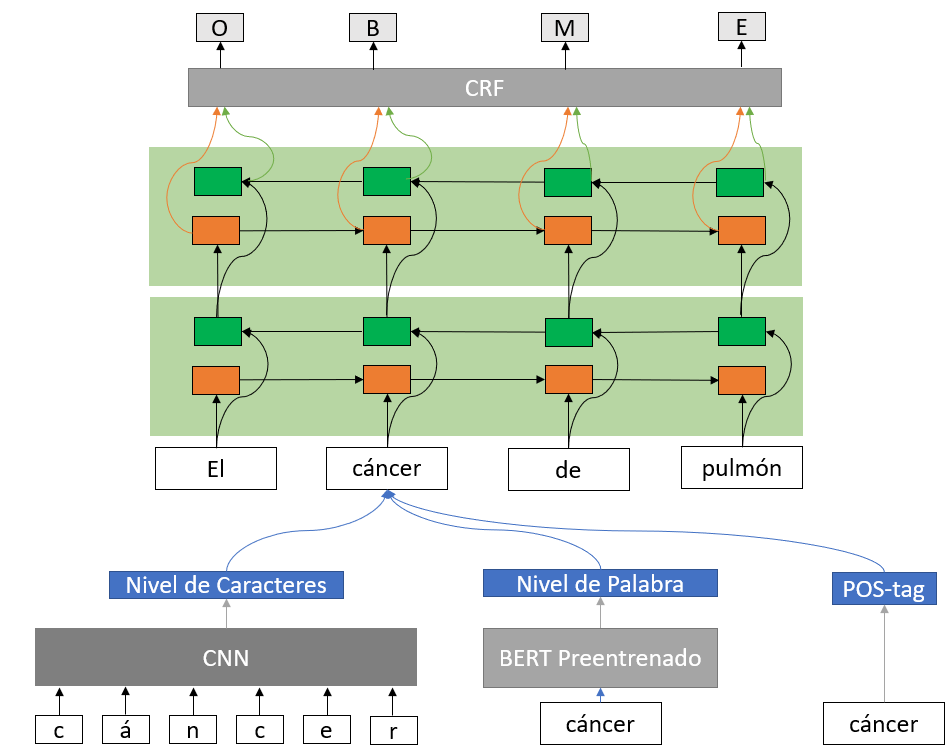
\includegraphics[width = 10cm]{Imagenes/EntitiesModelRec.png}
	\caption{Arquitectura del modelo de aprendizaje profundo para la extraccio\'on y clasificaci\'on de entidades con el CRF para la decodificaci\'on de las etiquetas \emph{BMEWO-V}.}\label{fig:ArcMod}
\end{figure}

\begin{figure}[h!]
	\centering
	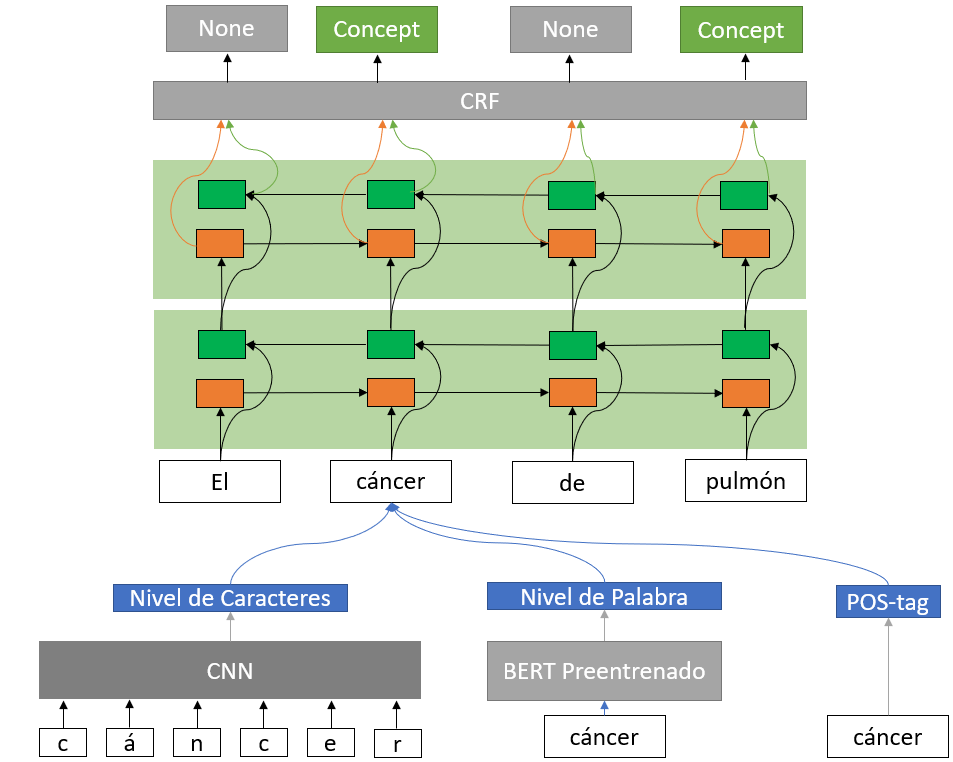
\includegraphics[width = 10cm]{Imagenes/EntitiesModelClas.png}
	\caption{Arquitectura del modelo de aprendizaje profundo para la extraccio\'on y clasificaci\'on de entidades con el CRF para la decodificaci\'on de las etiquetas de clasificaci\'on \emph{Concept}, \emph{Action}, \emph{Reference}, \emph{Predicate} y \emph{None},}\label{fig:ArcMod}
\end{figure}

En un primer nivel, el modelo se encarga de obtener la representaci\'on de cada token en la secuencia de entrada, para ello existe una capa intermedia que trabaja en funci\'on de transformar la caracter\'istica \emph{Char Indexes} en vectores, que junto al de \emph{PosTag} y el \emph{Embedding Contextual} forman la representaci\'on final del token. Una capa \textbf{CNN} convierte los \emph{Char Indexes} en un vector de \emph{embedding} que atrapa el significado sem\'antico del token a nivel de caracteres. Esto se incluye para que el modelo se auxilie de caracter\'isticas morfol\'ogicas de la palabra (como prefijos y sufijos) en caso de que el token no forme parte del vocabulario del \textbf{BERT} pre-entrenado. El vector obtenido a partir de la \textbf{CNN} concatenado con el vector de \emph{Embedding Contextual} y el de \emph{PosTag} forman la representaci\'on del token.

En un segundo nivel, el modelo procesa la secuencia de tokens para obtener representaciones a nivel de oraci\'on. Una capa \emph{Bi-LSTM} recorre la secuencia de tokens en ambos sentidos para construir dos secuencias de vectores. Los vectores en posiciones complementarias de las dos secuencias son concatenados, obteni\'endose as\'i nuevamente una secuencia que asocia un vector dependiente del contexto, que captura informaci\'on de la oraci\'on completa, a cada token de la oraci\'on. Esta secuencia busca atrapar las dependencias semánticas entre los tokens de la oración.
Luego una segunda \emph{Bi-LSTM} apilada, que se utiliza tradicionalmente para a\~nadir m\'as poder representacional, recorre la secuencia devuelta por la primera \emph{Bi-LSTM} en ambos sentidos, para tambi\'en construir dos secuencias de vectores que son concatenadas, produciendo as\'i otra nueva secuencia que asocia un vector a cada token de la oraci\'on capturando informaci\'on m\'as compleja que la obtenida por la primera capa \emph{Bi-LSTM}.

En el \'ultimo nivel, existen dos capas \emph{CRF} para la decodificaci\'on de etiquetas. La primera capa \emph{CRF} utiliza la representaci\'on obtenida del nivel anterior para predecir la secuencia de etiquetas \emph{BMEWO-V}. Mientras la segunda capa \emph{CRF} utiliza la representaci\'on obtenida del nivel anterior para predecir para cada token de la secuencia su clasificaci\'on como \emph{Concept}, \emph{Action}, \emph{Reference}, \emph{Predicate} y\emph{None} en caso que no sea ninguna de las anteriores.

\subsection{Postprocesamiento}
La primera capa de salida CRF produce una secuencia en el sistema de etiquetas $BMEWO$-$V$.
Las siglas responden a la nomenclatura: $B$ para inicio de una entidad, $M$ para palabras interiores, $E$ para palabras del final, $W$ para aquellas palabras que constituyen una entidad por sí mismas y O para las palabras que no forman parte de ninguna entidad.
También contempla la posibilidad de etiquetar palabras que pertecen a más de una entidad~(solapamiento de entidades), para lo cual incluye la etiqueta $V$.

Para extraer el conjunto de entidades presentes en la oración a partir de la salida de la primera capa CRF, se utiliza un proceso que será referido de ahora en adelante como \textbf{decodificación}.
La decodificación se complejiza debido a un elemento característico del problema descrito: las palabras pertenecientes a una misma entidad no aparecen necesariamente de manera contigua en la oración.
Por ejemplo, en la oración: \textit{La vitamina D también juega un rol en su sistema nervioso, muscular e inmunitario.}, extraída de la colección de entrenamiento del evento \textit{eHealth-KD 2019}, aparecen marcadas como relevantes las entidades \textit{sistema nervioso}, \textit{sistema muscular} y \textit{sistema inmunitario}; las dos últimas formadas por palabras no consecutivas en la oración.
Teniendo en cuenta esto, el proceso de decodificación se divide en dos etapas.
En una primera instancia se detectan y extraen el conjunto de entidades entre las que se encuentran todas aquellas que están formadas por palabras no contiguas~(entidades discontinuas); luego, se extraen todas aquellas formadas por \textit{tokens} adyacentes~(entidades continuas), tomando como premisa que no existe ninguna discontinua restante.

De acuerdo al uso correcto del idioma Español, se redujeron los escenarios donde pueden aparecer entidades discontinuas a las subsecuencias que se corresponden con las expresiones regulares: $(V^+)((M^*EO^*)+)(M^*E)$ y $((BO)^+)(B)(V^+)$.
La primera agrupa a las entidades que comparten los \textit{tokens} iniciales; la segunda, a aquellas que comparten las palabras finales.
Un ejemplo que se incluye en el primer grupo lo constituye el fragmento: \textit{cáncer de mama y de pulmón}, correctamente etiquetado como $VMEOME$, de donde se extraen las entidades \textit{cáncer de mama} y \textit{cáncer de pulmón}.
Como ejemplo del segundo grupo se puede citar el fragmento: \textit{tejidos y órganos humanos}, correctamente etiquetado como $BOBV$, de donde se extraen las entidades \textit{tejidos humanos} y \textit{órganos humanos}.
El proceso de decodificación de estos dos escenarios permite obtener satisfactoriamente las entidades discontinuas en las colecciones de entrenamiento y desarrollo con un error menor al $1\%$, asumiendo que las secuencias están etiquetadas correctamente.


Después de a detección de posibles entidades discontinuas, la segunda etapa comienza asumiendo que las restantes están formadas por secuencias continuas de palabras.
Para ello las etiquetas asociadas a todas las entidades extraídas en la primera etapa son cambiadas a $O$. 


Para extraer las entidades continuas se lleva a cabo un proceso iterativo sobre la secuencia de etiquetas.
Debido a las limitaciones del sistema $BMEWO$-$V$, también se asume que en una misma palabra no se solapan más de dos entidades.
Abandonar esta suposición no aporta mucha mayor información~\footnote{Cuando se dice que no aporta mucha mayor información se hace referencia al hecho de que no es común, de acuerdo a la evaluación que se realizó sobre las colecciones de entrenamiento y desarrollo, encontrar tres o más entidades solapadas en una misma palabra}, además de que se introduce ambigüedad en el proceso dada por la incertidumbre que habría en dicho caso con respecto al número de entidades a las que el \textit{token} en cuestión pertenecería.
Dado esto, a lo largo del procedimiento se matienen dos entidades en formación.
En cada iteración estas dos entidades son creadas, extendidas o emitidas de acuerdo con reglas definidas en una máquina que actúa de manera determinista en función solamente de la etiqueta actual y la anterior en la secuencia que se procesa.
La figura \ref{fig:automaton} resume la función de decisión de dicho autómata. 

\begin{figure}[h!]
	\centering
	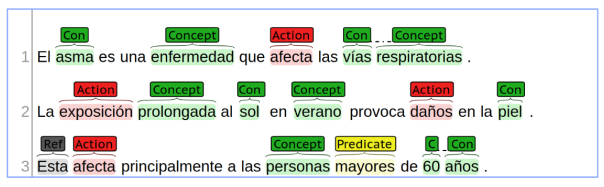
\includegraphics[width = 10cm]{Graphics/automaton.png}
	\caption{Función de decisión del autómata en la segunda etapa de la decodificación de la salida del modelo de extracción de entidades.}\label{fig:automaton}
\end{figure}

De acuerdo a evaluaciones efectuadas en las colecciones de entrenamiento y desarrollo, el proceso de decodificación de secuencias etiquetadas de manera correcta, extrae adecuadamente más del $98\%$ de las entidades presentes.


Luego de identificadas las entidades, para clasificar cada una de ellas de acuerdo a su tipo, se utiliza un sistema de votaci\'on, basado en la salida de la segunda capa CRF.
La misma asocia, para cada palabra en la oración de entrada, uno de los tipos de entidad, en este caso uno entre: \texttt{Concept}, \texttt{Action}, \texttt{Predicate} o \texttt{Reference}.
Cada palabra produce para cada entidad a la que pertenece, un voto de acuerdo al tipo que le fue asociado.
Luego, cada entidad se clasifica de según el tipo que mayor cantidad de votos que haya obtenido. Si está equilibrada la votación se asume \texttt{Concepto}, por ser la más frecuente por amplio margen en las colecciones estudiadas.




















%===================================================================================
% Chapter: Propuesta para la Extracción de Relaciones
%===================================================================================
\chapter{Propuesta para la Extracción de Relaciones}\label{chapter:relations}
\addcontentsline{toc}{chapter}{Extracción de Relaciones}

En este capítulo se hace una descripción de las técnicas empleadas para la resolución de la tarea de Extracción de Relaciones.
Primeramente, se recoge un resumen del análisis de dependencias de una oración, aspecto cardinal en la propuesta realizada.
Luego se describe el modelo de aprendizaje profundo propuesto, sus componentes y sus distintas variantes.


\section{Análisis de Dependencias}\label{sec:parsing}

El conocimiento de la estructura y la sintáxis que subyace en un texto en lenguaje natural puede ser de mucha ayuda en tareas típicas de NLP como la clasificación de texto, la sumarización o la extracción de relaciones.
Una de las técnicas más comunes para capturar cierta estructura en las oraciones es el análisis sintáctico~(conocido comúnmente por su nombre en inglés: \emph{parsing}).
En esta sección se abordará este tema, particularmente el análisis de dependencias.

Hay dos formas de describir la estructura de una oración en lenguaje natural: separando la oración en \textbf{constituyentes}~(frases), que se separan a su vez en constituyentes más pequeños; o estableciendo conexiones entre las palabras individuales~\cite{covington2001fundamental}.
El significado de estas dos variantes se ilustra en las figuras \ref{fig:dep_const} y \ref{fig:dep_links} respectivamente.

\begin{figure}[h!]
	\centering
	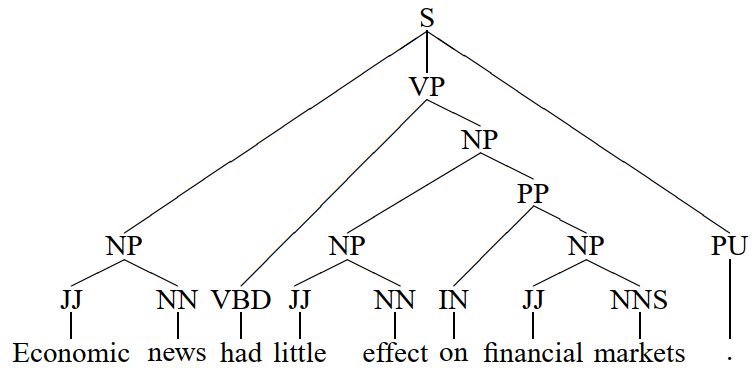
\includegraphics[width=0.8\linewidth]{Graphics/dep_const.png}
	\caption{Estructura constituyente para una oración en idioma inglés del \emph{Penn Treebank}.}\label{fig:dep_const}
\end{figure}

\begin{figure}[h!]
	\centering
	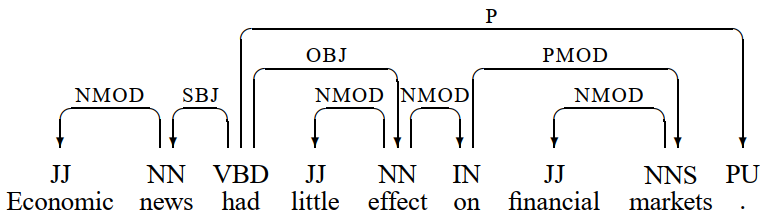
\includegraphics[width=0.8\linewidth]{Graphics/dep_links.png}
	\caption{Estructura de dependencias para una oración en idioma inglés del \emph{Penn Treebank}.}\label{fig:dep_links}
\end{figure}

La representación constituyente del lenguaje data de varios años atrás, y ha sido explotada tanto por los científicos de la computación como por lingüistas, en aras de obtener buenas representaciones del lenguaje natural.
Sin embargo, la comunidad científica ha mostrado un creciente interés en los últimos años en las estructuras de dependencias como una alternativa a esta representación.

La noción fundamental de \textbf{dependencia} está basada en la idea de que la estructura sintáctica de una oración está conformada por un conjunto de relaciones binarias asimétricas entre las palabras de dicha oración~\cite{nivre2005dependency}.
Siempre que se establece una relación entre dos palabras, a una de ellas se le denomina \textbf{cabecera} y a la otra \textbf{dependiente}.
A continuación se listan algunos criterios que han sido propuestos para identificar una relación sintáctica entre una cabecera $H$ y un dependiente $D$, en una construcción sintáctica $C$~\cite{zwicky1985heads, richard1990english}:

\begin{enumerate}
	\item $H$ determina la categoría sintáctica de $C$, y muchas veces puede sustituir a $C$.
	
	\item $H$ determina la categoría semántica de $C$, mientras que $D$ aporta especificidad.
	
	\item $H$ es obligatoria, mientra que $D$ es opcional.
	
	\item $H$ selecciona a $D$, y determina si puede o no ser opcional.
	
	\item La forma de $D$ depende de $H$.
	
	\item La posición de $D$ en la oración se especifica con respecto a $H$.
\end{enumerate}

Estas reglas no son absolutas y contienen un mezcla de criterios variados, algunos sintácticos, otros semánticos.
No existe en la literatura una noción coherente de dependencia que se corresponda con todos los distintos criterios~\cite{nivre2005dependency}.


\subsection{Grafo de dependencias}

Si se considera cada dependencia como un arco dirigido que tiene como origen a la cabecera y como destino al dependiente, la estructura de dependecias de la oración conforma un grafo dirigido $G$ cuyos nodos son los elementos léxicos del lenguaje~(\emph{tokens}).
Además, el grafo subyacente de $G$ debe estar conectado, para que cada nodo esté relacionado con, al menos, otro nodo.

A esta caracterización se le imponen usualmente más restricciones.
Dos de las más utilizadas en las distintas formalizaciones de gramáticas basadas en dependencias~(o simplemente, gramáticas de dependencias), son: la suposición de que cada nodo del grafo tiene \emph{indegree} $\leq 1$; y la no existencia de ciclos.
Estas suposiciones, junto a la consideración de conectividad, implican que este grafo sea un árbol dirigido con una sola raíz la cual no depende de ninguna otra palabra.
Esto último queda ilustrado en la figura \ref{fig:dep_tree}.
A esta estructura se le denomina \textbf{árbol de dependencias}.

\begin{figure}[h!]
	\centering
	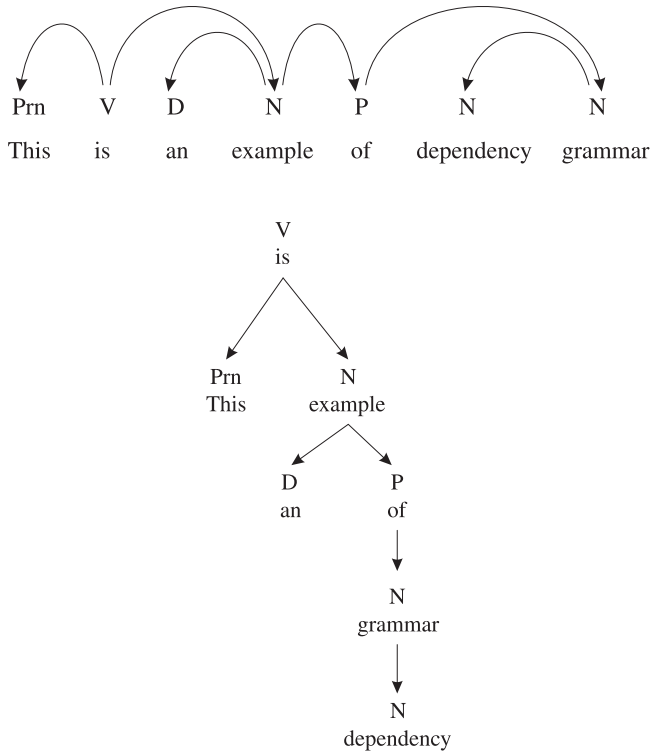
\includegraphics[width=0.7\linewidth]{Graphics/dep_tree.png}
	\caption{Estructura de dependencias para una oración en idioma inglés y árbol de dependencias.}\label{fig:dep_tree}
\end{figure}

Existen varias restricciones adicionales que se definen sobre estas estructuras y que son más debatidas.
Una de las más conocidas es la restricción de \textbf{proyectividad}~\cite{hays1964dependency,lecerf1960programme,marcus1965notion}.
Un grafo de dependencias satisface la restricción de proyectividad con respecto a un orden linear particular de los nodos si, por cada arco $h \rightarrow d$ y un nodo $w$, $w$ ocurre entre $h$ y $d$ en el orden lineal solo si $w$ está \textbf{dominado} por $h$~\footnote{La relación \textbf{dominar} es la clausura reflexiva y transitiva de la relación de dependencia definida por los arcos}. 

\section{Modelo de Aprendizaje Profundo}\label{sec:model}

El modelo de aprendizaje profundo propuesto se apoya en el uso de RNN sobre estructuras derivadas del árbol de dependencias de la oración de entrada y las entidades señaladas, para obtener una representación de la supuesta relación existente entre ellas.

\subsection{Hipótesis del Camino en el Árbol de Dependencias}

Como fue explicado en el capítulo~\ref{chapter:information_extraction}, la información más completa para resolver el problema de la extracción de relaciones se encuentra en la oración completa. Sin embargo, se maneja por muchos autores la suposición de que el árbol de dependencias de la oración de entrada condensa la información vital para resolver el problema, a la vez que desecha otras fuentes de desinformación.

El hecho de que las entidades entre las cuales se quiere determinar la existencia de una relación estén formadas por múltiples palabras, constituye un problema para la configuración de algoritmo de aprendizaje profundo.
Es factible, en términos de implementación, concebir una configuración que permita establecer la existencia de relaciones entre dos palabras o \textit{tokens} de la oración.
Pero si las entidades están formadas por múltiples palabras, un aspecto cardinal de la implementación consiste en definir qué palabra va a \textit{representar} a la entidad a la hora de determinar las relaciones en las que participa.
Con este fin se han explorado diversos criterios en la literatura.
Se debate el uso de la última palabra de la entidad en algunos casos; en otros, de la primera.
De manera general, de acuerdo a observaciones realizadas sobre el conjunto de datos estudiado, las entidades señaladas constituyen unidades sintácticas coherentes; llegando a ser sintagmas nominales completos, en varios ejemplos.
Como fue abordado, uno de los criterios que determina la existencia de una dependencia con una cabecera \textit{H} en una construcción sintáctica \textit{C}, es que \textit{H} puede sustituir sintácticamente a \textit{C}.
Incluso, \textit{H} puede determinar semánticamente a \textit{C}.
Por otro lado, las entidades formadas por múltiples palabras suelen ocurrir de manera total en un subárbol del árbol de dependencias, que tiene como raíz una de las palabras de la entidad.
Este hecho fue explorado en el conjunto de datos estudiado, y se cumple en la amplia mayoría de los casos, exceptuándose muy pocos ejemplos.
Dicho subárbol correspondiente a una entidad \textit{e} lo definimos como \textbf{subárbol relevante a \textit{e}}, y lo denotamos como $S_e$.
A la raíz de dicho subárbol la denominamos \textbf{núcleo de la entidad $e$}, y se denota como $n_e$.

Otra definición importante, citada repetidamente en la literatura para resolver este problema es el \textbf{camino en el árbol de dependencias} entre dos \textit{tokens} $t_1,t_2$.
Esta definición es intuitiva, y denota a la secuencia de \textit{tokens} que ocurren en el camino que va desde $t_1$ hasta $t_2$.
Dicho camino será denotado como $C(t_1,t_2)$.

La figura \ref{fig:dep_tree_ex} ilustra las definiciones anteriores.

\begin{figure}[h!]
	\centering
	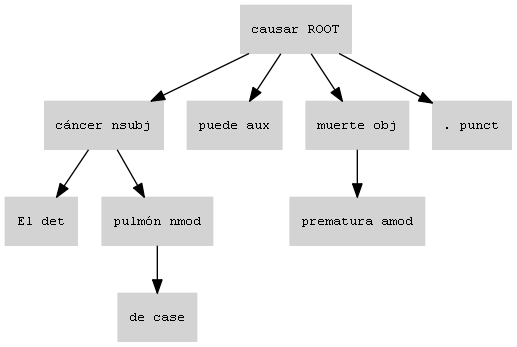
\includegraphics[width=0.7\linewidth]{Graphics/dep_tree_ex.png}
	\caption{Árbol de dependencias de la oración: \textbf{El cáncer de pulmón puede causar muerte prematura}. Se establece la relación \textbf{entails} entre las entidades \textbf{cáncer de pulmón}($e_1$) y \textbf{muerte}($e_2$). Aparecen señalados $S_{e_1}$, $S_{e_2}$, así como $C(n_{e_1}, n_{e_2})$.}\label{fig:dep_tree_ex}
\end{figure}

En la selección del modelo propuesto se consideran dos hipótesis fundamentales a la hora de establecer la existencia de una relación entre dos entidades $e_1,e_2$, las cuales se comprobaron de manera experimental, como será descrito en el capítulo \ref{chapter:experiments}:

\begin{enumerate}
	\item $S_{e_1}$ y $S_{e_2}$ condensan información útil sobre las respectivas entidades, a la vez que deshechan fuentes de desinformación.
	
	\item $C(n_{e_1}, n_{e_2})$ condensa información útil para determinar una posible relación entre $e_1$ y $e_2$, a la vez que deshecha fuentes de desinformación.
\end{enumerate}


\subsection{Red Neuronal}

La configuración de red definida, pretende determinar la existencia de una relación entre las entidades $e_1$ y $e_2$ en el contexto de una oración dada. Para ello codifica la información contenida en los subárboles relevantes a $e_1$ y $e_2$~(denotados $S_{e_1}$ y $S_{e_2}$, respectivamente), así como en el camino en el árbol de dependencias entre los núcleos de $e_1$ y de $e_2$~(denotado $C(n_{e_1}, n_{e_2})$).

Tanto $S_{e_1}$, $S_{e_2}$ como $C(n_{e_1}, n_{e_2})$, son estructuras formadas por palabras de la oración de entrada. Para representar las palabras de la oración en cada una de estas estructuras, se utiliza un vector que se obtiene a partir de la concatenación de \textit{embeddings} provenientes de distintas fuentes de información:

\begin{description}
	\item[\textit{Embedding} Contextual:] Se utilizan \textit{embeddings} contextuales preentrenados, obtenidos a partir del modelo BERT.
	
	\item[\textit{Embedding} de Palabras:] Se utilizan \textit{embeddings} preentrenados en un corpus construido a partir de artículos de Wikipedia con contenido médico.
	
	\item[Caracteres:] Se utilizan \textit{embeddings} obtenidos mediante una CNN sobre los caracteres de la palabra.
	
	\item[POST-tag y Dependencia:] Se utiliza un \textit{embedding} de la etiqueta de POS-tag de la palabra y la dependencia de la misma con su ancestro en el árbol de dependencias de la oración.
	
	\item[Etiqueta BMEWO-V y Tipo de la entidad:] Se añaden \textit{embeddings} con información relativa a la entidad a la que pertenece la palabra en cuestión.
	En este caso la etiqueta correspondiente en el sistema BMEWO-V así como el tipo de la entidad.
	
\end{description}

Para la obtención de los \textit{embedding} contextuales se utilizó el modelo preentrenado \textbf{tal y poner cita}.
Los \textit{embedding} de palabras fueron entrenados utilizado el algoritmo \textbf{word2vec}\cite{word2vec} con la arquitectura \textbf{skipgram}.
Las etiquetas de POS-tag así como el árbol de dependecias fueron obtenidos utilizando la biblioteca \textbf{spaCy}\cite{spacy2}.
En el caso de las etiquetas BMEWO-V y los tipos de las entidades se obtienen a partir de las salidas del modelo de extracción de entidades descrito en el capítulo \ref{chapter:entities}.

A partir de las estructuras $S_{e_1}$, $S_{e_2}$ y $C(n_{e_1}, n_{e_2})$, se obtiene una representación de la oración y las entidades señaladas.
Una capa BiLSTM transforma la representación de cada palabra de la secuencia $C(n_{e_1}, n_{e_2})$, para incluir información contextual de las palabras anteriores y posteriores de cada posición.

\begin{equation*}
	P = BiLSTM(C(n_{e_1}, n_{e_2}))
\end{equation*}

Luego, la capa LSTM apilada enfatiza la direccionalidad de la supuesta relación, procesando la secuencia $P$ solamente en el sentido que va desde el origen hacia el destino de la misma, y obtiene un vector $p$ que codifica la información contenida en $C(n_{e_1}, n_{e_2})$.

\begin{equation*}
p = LSTM(P)
\end{equation*}

Entre tanto, una capa recurrente se aplica sobre $S_{e_1}$ y $S_{e_2}$ de manera independiente~\footnote{Las representaciones de $S_{e_1}$ y $S_{e_2}$ se obtienen de manera independiente, pero utilizando el mismo conjunto de parámetros.}.
En este caso se utiliza una red Tree-LSTM, en su variante $Child Sum$~\cite{treeLSTM}.

\begin{equation*}
	t_{e_1} = TreeLSTM(S_{e_1})
\end{equation*}


\begin{equation*}
	t_{e_2} = TreeLSTM(S_{e_2})
\end{equation*}


Una red Tree-LSTM es una generalización de una red LSTM, que permite procesar de manera recurrente estructuras de vectores que se organicen en forma de grafos dirigidos y acíclicos~(como los árboles, por ejemplo).

Una celda Tree-LSTM en el momento $t$, al igual que su homólogo lineal, se define como una colección de vectores en $\mathbb{R}^d$, siendo $d$ la dimensión oculta de dicha celda.
Estos vectores son: una compuerta de entrada $i_t$, una compuerta de olvido $f_t$, una compuerta de salida $o_t$, una celda de memoria $c_t$ y un estado oculto $h_t$. Siendo $C(j)$ la secuencia de hijos de el nodo $j$, las ecuaciones de transición de una celda Tree-LSTM se muestran a continuación:

\begin{equation*}
	\overline{h}_j = \sum_{k\in C(j)} h_k
\end{equation*}

\begin{equation*}
i_j = \sigma(W^{(i)}x_j + U^{(i)}\overline{h}_j + b(i))
\end{equation*}

\begin{equation*}
f_{jk} = \sigma(W^{(f)}x_j + U^{(f)}h_k + b(f))
\end{equation*}

\begin{equation*}
o_j = \sigma(W^{(o)}x_j + U^{(o)}\overline{h}_j + b(o))
\end{equation*}

\begin{equation*}
u_j = tanh(W^{(u)}x_j + U^{(u)}\overline{h}_j + b(u))
\end{equation*}

\begin{equation*}
c_j = i_j \odot u_j + \sum_{k\in C(j)} f_{jk} \odot c_k
\end{equation*}

\begin{equation*}
h_j = o_j \odot tanh(c_j)
\end{equation*}

Nótese que la diferencia con respecto a las redes LSTM radica en que, como se tienen varios momentos inmediatos anteriores al momento $t$, se considera la suma de todos los respectivos estados ocultos. La figura \ref{fig:lstm_cmp} ilustra las diferencias entre ambas.

\begin{figure}[h!]
	\centering
	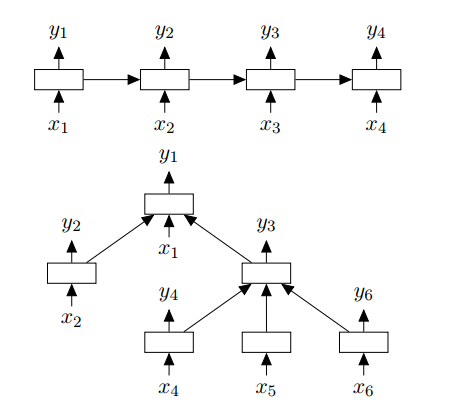
\includegraphics[width=0.7\linewidth]{Graphics/lstm_cmp.png}
	\caption{\textbf{Arriba}: LSTM tradicional o de cadena. \textbf{Abajo}: Tree-LSTM~\cite{treeLSTM}.}\label{fig:lstm_cmp}
\end{figure}

Loa vectores obtenidos a partir de la secuencia de entrada y las entidades señaladas se concatenan para formar la representación de la hipotética relación.

\begin{equation*}
	r = [t_{e_1};t_{e_2}, p]
\end{equation*}

La salida $x$ se obtiene a partir de aplicar la función sigmoide a una transformación linear de dicho vector.

\begin{equation*}
	x = \sigma(W^{(x)}r + b^{(x)})
\end{equation*}

La matriz $W^{(x)}$ tiene dimensiones $m \times l$, donde $l = |t_{e_1}| + |t_{e_2}| + |p|$ y $m$ es el número de relaciones semánticas diferentes que se definen.

De acuerdo al vector de salida $x$, se predice la existencia de una relación si su valor máximo excede un umbral prefijado que se introduce como un hiperparámetro adicional. De ser así, se predice la existencia solamente de la relación dada por $\arg\max(x)$.
	
Nótese como, a diferencia de las arquitecturas tradicionales, esta configuración permite prescindir de la relación ficticia \textit{none}.

La figura \ref{fig:rel_model} ilustra la arquitectura descrita.

\begin{figure}[h!]
	\centering
	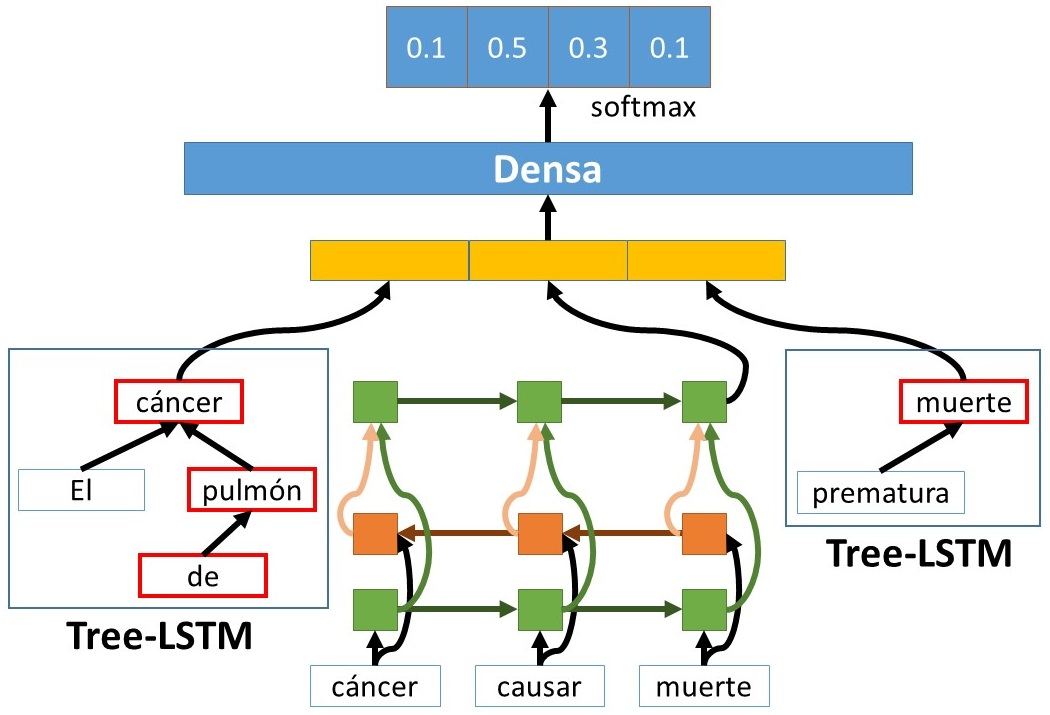
\includegraphics[width=1\linewidth]{Graphics/rel_model_class.jpg}
	\caption{Arquitectura de red utilizada. La oración de entrada es \textbf{El cáncer de pulmón puede causar muerte prematura} Y las entidades en cuestión son \textbf{cáncer de pulmón} y \textbf{muerte}.}\label{fig:rel_model}
\end{figure}

\section{Entrenamiento}

Debido a que la salida correspondiente a cada relación es independiente de las otras, el modelo se entrena para minimizar una función de entropía binaria.
Siendo $k$ el número de relaciones definidas, la función de pérdida entre la salida del modelo $x$ y un vector binario $y$ objetivo, se define como:

\begin{equation*}
	\ell(x, y) = \frac{1}{k}\sum_{1\leq i\leq k}{\left[ y_i \cdot \log x_i + (1 - y_i) \cdot \log (1 - x_i) \right]}
\end{equation*}

Como fue explicado, la salida del modelo no expresa directamente la existencia de una relación ficticia que contemple el caso de la no existencia de relación entre el par de entidades de entrada.
Para que el modelo sea capaz de reconocer estos casos, se introduce una estrategia de muestreo negativo durante el entrenamiento, donde el vector objetivo es el vector nulo.
Dicho muestreo no se realiza utilizando como entrada pares de palabras aleatorios, sino núcleos de entidades existentes en la oración entre las cuales no existe una relación.
En el capítulo \ref{chapter:experiments} se describirán experimentos realizados con distintas estrategias de muestreo negativo utilizadas.

%===================================================================================
%===================================================================================
% Chapter: Análisis Experimental
%===================================================================================
\chapter{Análisis Experimental}\label{chapter:experiments}
\addcontentsline{toc}{chapter}{Análisis Experimental}

Este capítulo se centra en la descripción de los detalles de la implementación de las propuestas descritas para la extracción de entidades y relaciones.
Se explican las configuraciones de los exprimentos realizados y el conjunto de técnicas experimentales empleadas, se muestran los resultados de dicho estudio y se someten los mismo a una posterior discusión.

\section{Marco Experimental}

El desarrollo de los experimentos de este trabajo se enmarca en el evento \textit{eHealth Knowledge Discovery Challenge}, en sus ediciones de 2019 y 2020.
En la misma, los problemas de extracción de entidades y relaciones están organizados en dos tareas.

\begin{description}
	\item[Tarea A:] Extracción y clasificación de entidades.
	Es objetivo de esta tares es, dada una lista de documentos~(oraciones) en idioma Español con contenido médico, extraer las entidades relevantes presentes en dicho documento, y clasificarlas de acuerdo al tipo de concepto que representan~(\texttt{Concept}, \texttt{Action}, \texttt{Predicate} o \texttt{Reference}).
	Las entidades son conceptos semánticamente importantes dentro de una oración.
	Pueden estar formadas por una o varias palabras, las cuales no necesariamente aparecen de manera continua en el texto de la oración.
	La figura \ref{fig:entites_ex} muestra las entidades relevantes que aparecen en un conjunto de oraciones de ejemplo.
	
	La entrada de la Tarea A es un documento de texto con una oración	por línea.
	La salida es una colección de entidades, con un identificador numérico asociado a cada una.
	Cada entidad esta constituída por una lista de segmentos del texto \texttt{<inicio, fin>}, que representan las palabras por las que está conformado dicho concepto.
	
	\item[Tarea B:] Extracción de relaciones.
	La Tarea B parte del conjunto de entidades obtenido en la Tarea A.
	El objetivo de esta tarea es indentificar las relaciones semánticas relevantes entre los conceptos encontrados en cada oración.
	Ocho de las trece relaciones semánticas presentes en los conjuntos de datos pueden ser observadas en la figura \ref{fig:relations_ex}.
		
	La entrada de la Tarea B es un documento de texto con una oración	por línea, y una colección de entidades, con su correspondiente identificador numérico y etiqueta.
	La salida de la Tarea B es una lista de tuplas de la forma \texttt{<id1,id2,rel>} que denota la existencia de una relación con origen en la entidad con identificador \texttt{id1}, y destino en \texttt{id2}, y que se le asigna el tipo \texttt{rel}.
	
\end{description} 
	
\begin{figure}[h!]
	\centering
	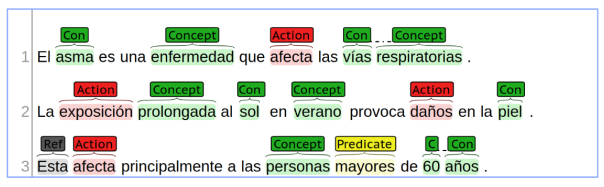
\includegraphics[width=0.9\linewidth]{Graphics/entities.png}
	\caption{Anotación de las entidades relevantes y sus respectivas clases en un conjunto de oraciones de ejemplo.} \label{fig:entites_ex}
\end{figure}

\begin{figure}[h!]
	\centering
	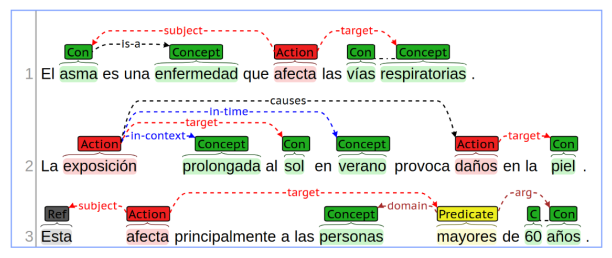
\includegraphics[width=0.9\linewidth]{Graphics/relations.png}
	\caption{Anotación de las relaciones semánticas relevantes en un conjunto de oraciones de ejemplo.} \label{fig:relations_ex}
\end{figure}


\subsection{Escenarios de Evaluación}\label{subsec:eval_sce}

El concurso propone un escenario de evaluación principal (Escenario 1) donde las dos tareas descritas anteriormente se realizan de forma secuencial.
Adicionalmente, los participantes tuvieron la oportunidad de enfocarse en una de las dos tareas específicamente, a partir de entregar resultados en dos escenarios opcionales, uno para cada tarea.
Estos dos escenarios adicionales miden el rendimiento en tareas individuales de forma independiente entre ellas.

\begin{description}
	
\item[Escenario 1 [A+B]:] Recibe como entrada un conjunto de oraciones a anotar.
El sistema produce tanto las instancias concretas de entidades
presentes en la colección como las relaciones existentes entre ellas.
El rendimiento general del sistema se mide en función
del rendimiento en ambas tareas, según se describe en la sección 4.1.2.
 
\item[Escenario 2 [A]:] Recibe como entrada un conjunto de oraciones a anotar.
El sistema produce únicamente el conjunto de entidades presentes en la colección (con la correspondiente clasificación según el tipo de concepto que representa).

\item[Escenario 3 [B]:] Recibe como entrada un conjunto de oraciones y una colección de entidades anotadas y etiquetadas en el texto.
El sistema produce únicamente el conjunto de relaciones que existen entre las instancias concretas de los conceptos.

\item[Escenario 4 [A+B~(Dominio General)]:] Este escenario fue incluido como una novedad en el evento del año 2020.
Es similar al Escenario 1 de evaluación, pero considera oraciones cuyo contenido es de dominio general.

\end{description}

\subsection{Métricas de Evaluación}

La métrica de evaluación es la medida \textit{F1} estándar, donde la precisión y recobrado se definen en términos de coincidencias \textbf{[C]orrectas}, \textbf{[I]ncorrectas},
\textbf{[P]arciales}, \textbf{[F]altantes} y \textbf{[S]obrantes}.


\begin{description}
	
	\item[Anotación correcta:] Reportada cuando una palabra clave es encontrada cuya sección de texto (secuencia de tuplas \texttt{<INICIO, FIN>}) coincide	exactamente con la de una en el corpus de referencia.
	Solo una coincidencia correcta por entrada en la colección de referencia puede ser reportada.
	Por tanto, las entradas duplicadas cuentan como Sobrantes.
	
	\item[Anotación incorrecta:] Reportada cuando una entidad es identificada correctamente en lo que a sección de texto respecta, pero no le fue asignado el tipo de concepto correcto.
	
	\item[Anotación parcial:] Reportada cuando dos intervalos \texttt{<INICIO, FIN>} tienen una intersección no vacía, como es el caso de “vías respiratorias”	y “respiratorias”.
	Notar que una anotación parcial es considerada solo sobre una única anotación correcta en la colección de referencia.
	
	\item[Anotación faltante:] Aquellas anotaciones que aparecen en la colección de	referencia pero no en la respuesta.
	
	\item[Anotación sobrante:] Aquellas anotaciones que aparecen en la respuesta pero no en la colección de referencia.
	
\end{description}

A las coincidencias parciales se les asigna la mitad de la
puntuaciones de las coincidencias correctas, mientras que a las anotaciones faltantes y sobrantes no se les da puntos.
Las fórmulas de evaluación para el Escenario 1 se definen de la siguiente forma:

\begin{equation*}
P = \frac{C_A + \frac{1}{2}P_A + C_B}{C_A + I_A + P_A + S_A + C_B + S_B}
\end{equation*}

\begin{equation*}
R = \frac{C_A + \frac{1}{2}P_A + C_B}{C_A + I_A + P_A + F_A + C_B + F_B}
\end{equation*}

\begin{equation*}
F1 = 2\frac{PR}{P+R}
\end{equation*}

Siendo $P$ y $R$ los valores de precisión y recobrado respectivamente.

Análogamente, se definen fórmulas similares para los escenarios 2 y 3, pero usando solo las estadísticas de la tarea A y B, respectivamente.

\subsection{Corpus de Evaluación}


\subsection{Implementación y Bibliotecas Externas}

La implementación de las propuestas se realizó utilizando el lenguaje de programación Python.
Se utilizó la biblioteca \texttt{PyTorch} como marco para el trabajo con redes neuronales profundas.
Para la obtención de los \textit{embedding} contextuales se utilizó una variente del modelo \texttt{BERT}~\cite{devlin2018bert}, en este caso: \texttt{bert-base-multilingual-uncased}, a través de la interfaz que brinda la biblioteca \texttt{pytorch-pretrained-bert}~\footnote{https://pypi.org/project/pytorch-pretrained-bert/}.
Los \textit{embeddings} de palabras fueron entrenados utilizado el algoritmo \texttt{word2vec}~\cite{mikolov2013efficient} con la arquitectura \texttt{skipgram}, utilizando la interfaz de la biblioteca \texttt{gensim}~\footnote{https://pypi.org/project/gensim/}.
Las etiquetas de POS-tag así como el árbol de dependencias fueron obtenidos utilizando la biblioteca \texttt{spaCy}~\footnote{https://spacy.io/}.

\subsection{Infraestructura Computacional}



\subsection{Entrenamiento y Ajuste de Parámetros}\label{sec:training}

Los algoritmos definidos para la resolución de ambas tareas, están basados en técnicas de aprendizaje profundo.
Una de las implicaciones de esta decisión, es que una vez fijo el algoritmo, existe una amplia variedad de hiperparámetros que se pueden ajustar en virtud de obtener mejores resultados computacionales.

Las tablas \ref{table:params_taskA} y \ref{table:params_taskB} describen las configuraciones de parámetros utilizadas cada uno de los modelos y para su entrenamiento.

\begin{table*}[tb]\centering
		\begin{tabular}{lc}
			\hline
			\textbf{Parámetro} & \textbf{Valor} \\
			\hline
			\hline
			\multicolumn{2}{c}{\textbf{Entradas}}\\
			\hline
			\hline
			Dim. del \textit{embedding} contextual & 9216~(12 capas)\\
			Dim. del \textit{embedding} de palabras & 300\\
			Dim. del \textit{embedding} de caracteres & 100\\
			Dim. del \textit{embedding} de POS-tag & 100\\
			
			\hline
			\hline
			\multicolumn{2}{c}{\textbf{Red neuronal}}\\
			\hline
			\hline
			
			Dimensión de la BiLSTM & 300\\
			
			\hline
			\hline
			\multicolumn{2}{c}{\textbf{Entrenamiento}}\\
			\hline
			\hline
			
			Optimizador & Adam\\
			\textit{Learning rate} & 0.001\\
			Épocas & 20\\
			
			\hline
			\hline
			
			\textbf{Total de parámetros} & X\\
			
			\hline
			
		\end{tabular}
	
	\caption{Configuración de parámetros del modelo de extracción de entidades. \textbf{[Arriba]} Red neuronal. \textbf{[Abajo]} Entrenamiento.}\label{table:params_taskA}
	
\end{table*}

\begin{table*}[tb]\centering
	\begin{tabular}{lc}
		\hline
		\textbf{Parámetro} & \textbf{Valor} \\
		\hline
		\hline
		\multicolumn{2}{c}{\textbf{Entradas}}\\
		\hline
		\hline
		Dim. del \textit{embedding} contextual & 768~(última capa)\\
		Dim. del \textit{embedding} de palabras & 300\\
		Dim. del \textit{embedding} de caracteres & 50\\
		Dim. del \textit{embedding} de POS-tag & 50\\
		Dim. del \textit{embedding} de dependencias & 50\\
		Dim. del \textit{embedding} de las etiquetas BMEWO-V & 50\\
		Dim. del \textit{embedding} del tipo de entidad & 50\\
		
		\hline
		\hline
		\multicolumn{2}{c}{\textbf{Red neuronal}}\\
		\hline
		\hline
		
		Dimensión de la BiLSTM & 100\\
		Dimensión de la Tree-LSTM & 50\\
		
		\hline
		\hline
		\multicolumn{2}{c}{\textbf{Entrenamiento}}\\
		\hline
		\hline
		
		Optimizador & Adam\\
		\textit{Learning rate} & 0.001\\
		Épocas & 30\\
		Muestreo negativo & 300\% de ej. positivos\\
		
		\hline
		\hline
		
		\textbf{Total de parámetros} & X\\
		
		\hline
		
	\end{tabular}
	
	\caption{Configuración de parámetros del modelo de extracción de relaciones. \textbf{[Arriba]} Red neuronal. \textbf{[Abajo]} Entrenamiento.}\label{table:params_taskB}
	
\end{table*}
		
Fueron entrenados modelos para ser evaluados tanto en el contexto del evento \textit{eHealth-KD} 2019, como en la edición del presente año.
En cada caso, la optimización de los modelos se realizó utilizando la colección de entrenamiento proveída a los concursantes.
El entrenamiento fue acompañado de un procedimiento de validación cruzada, que permitió determinar un número conveniente de épocas de entrenamiento, ajustar la complejidad de los modelos, así como seleccionar los más efectivos para someterlos a evaluación; para lo cual se utilizó la respectiva colección de desarrollo.


\section{Resultados Computacionales}

Los modelos fueron evaluados en los distintos escenarios de los evento \textit{eHealth-KD} 2019 y en su edición del 2020. La tabla \ref{table:results_20} muestra los resultados en el evento del año 2020 en los distintos escenarios de evaluación. Por su parte, en la tabla \ref{table:results_19} se compara la propuesta con los sistemas participantes en la edición de 2019. En ambos casos aparecen resaltados los resultados de nuestro modelo.

\begin{table*}[tb!]\centering
	
	\begin{tabular}{|c|c|c|c|c|}
		\hline
		&  \multicolumn{4}{c|}{\textbf{Escenarios (Medida $F_1$)}} \\
		\hline
		\textbf{Equipo} & \textbf{1 (A+B)} & \textbf{2 (A)} & \textbf{3 (B)} &  \textbf{4 (A+B transfer)}\\
		\hline
		Vicomtech & 0.6655 & 0.8208 & 0.5832 & 0.5632 \\
		Talp-UPC & 0.6266 & 0.8158 & 0.5747 & 0.5835  \\
		\textbf{UH-MAJA-KD} & \textbf{0.6250} & \textbf{0.8143} & \textbf{0.5987} & \textbf{0.5477} \\
		IXA-NER-RE & 0.5574 & 0.6918 & 0.633235 & 0.4788 \\
		UH-MatCom &	0.5568 & 0.7949 & 0.5450 & 0.37307 \\
		SINAI &	0.4206 & 0.8252 & 0.4617 & 0.28125 \\
		HAPLAP & 0.3951 & 0.5419 & 0.3164 & 0.1377 \\
		baseline & 0.3951 & 0.5419 & 0.1313 & 0.1377 \\
		ExSim &	0.2456 & 0.3142 & 0.1313 & 0.1222 \\
		\hline
	\end{tabular}
	\caption{Resultados (medida $F_1$) en cada escenario, ordenados por el Escenario 1 en el evento \textit{eHealth-KD} 2020.\label{table:results_20}}
\end{table*}

\begin{table*}[tb!]\centering
	 
	\begin{tabular}{|c|c|c|c|}
		\hline
		&  \multicolumn{3}{c|}{\textbf{Escenarios (Medida $F_1$)}} \\
		\hline
		\textbf{Equipo} & \textbf{1 (A+B)} & \textbf{2 (A)} & \textbf{3 (B)} \\
		\hline
		TALP	          	   &  0.6394 &  0.8203 &  0.6269 \\
		coin\_flipper (ncatala) & 0.6218 &  0.7873 &  0.4933 \\	
		LASTUS-TALN (abravo)   & 0.5816 &  0.8167 &  0.2298	\\
		NLP\_UNED               & 0.5473 &  0.7543 &  0.5337 \\
		Hulat-TaskAB           & 0.5413 &  0.7758 &  0.1231 \\	
		\textbf{UH-MAJA-KD}    & \textbf{0.5189} &  \textbf{0.8156} &  \textbf{0.4336} \\	
		lsi2\_uned              & 0.4934 &  0.7315 &  0.1231	\\
		IxaMed                 & 0.4869 &  0.6825 &  0.4356 \\
		baseline               & 0.4309 &  0.5466 &  0.1231 \\
		Hulat-TaskA            & 0.4309 &  0.7903 &  0.1231 \\	
		VSP             	   & 0.4289 &  0.5466 &  0.4933 \\	
		\hline
	\end{tabular}
	\caption{Resultados (medida $F_1$) en cada escenario, ordenados por el Escenario 1 en el evento \textit{eHealth-KD} 2019.\label{table:results_19}}
\end{table*}

\subsection{Resultados por Escenarios de Evaluación}

A continuación se profundiza en el desempeño de la propuesta en los escenarios, no solo en términos de medida $F1$, sino también de precisión y recobrado.
Las tablas \ref{table:results_20_escenario1}, \ref{table:results_20_escenario2}, \ref{table:results_20_escenario3}, \ref{table:results_20_escenario4} resumen los resultados obtenidos en los disintos escenarios evaluativos en el evento \textit{eHealth-KD 20020}.

\begin{table*}[tb!]\centering
	\begin{tabular}{|c|c|c|c|}
		\hline
		&  \multicolumn{3}{c|}{\textbf{Escenario 1 (A + B)}} \\
		\hline
		\textbf{Equipo} & \textbf{F1} & \textbf{Precision} & \textbf{Recobrado} \\
		\hline
		Vicomtech & 0.665564 & 0.679364 & 0.652315  \\
		Talp-UPC & 0.626679 & 0.626969 & 0.626389 \\
		\textbf{UH-MAJA-KD} & \textbf{0.625} & \textbf{0.634542} & \textbf{0.615741} \\
		IXA-NER-RE & 0.55748 & 0.58008 & 0.536574 \\
		UH-MatCom & 0.556876 & 0.716157 & 0.455556 \\
		SINAI & 0.42069 & 0.651456 & 0.310648 \\
		HAPLAP & 0.395153 & 0.458435 & 0.347222 \\
		baseline & 0.395153 & 0.458435 & 0.347222 \\
		ExSim & 0.245644 & 0.312589 & 0.202315 \\	
		\hline
	\end{tabular}
	\caption{Resultados en escenario 1 en cuanto a medida F1, Precisi\'on y Recobrado \textit{eHealth-KD} 2020. \label{table:results_20_escenario1}}
\end{table*}


\begin{table*}[tb!]\centering
	\begin{tabular}{|c|c|c|c|}
		\hline
		&  \multicolumn{3}{c|}{\textbf{Escenario 2 (A)}} \\
		\hline
		\textbf{Equipo} & \textbf{F1} & \textbf{Precision} & \textbf{Recobrado} \\
		\hline
		SINAI & 0.825207 & 0.844633 & 0.806655 \\
		Vicomtech & 0.820882 & 0.821622 & 0.820144 \\
		Talp-UPC & 0.815836 & 0.807218 & 0.82464 \\
		\textbf{UH-MAJA-KD} & \textbf{0.814312} & \textbf{0.820255} & \textbf{0.808453} \\
		UH-MatCom & 0.794967 & 0.824952 & 0.767086 \\
		IXA-NER-RE & 0.6918 & 0.726733 & 0.660072 \\
		HAPLAP & 0.541978 & 0.503864 & 0.586331 \\
		baseline & 0.541978 & 0.503864 & 0.586331 \\
		ExSim & 0.314214 & 0.292117 & 0.339928 \\	
		\hline
	\end{tabular}
	\caption{Resultados en escenario 2 en cuanto a medida F1, Precisi\'on y Recobrado \textit{eHealth-KD} 2020. \label{table:results_20_escenario2}}
\end{table*}

\begin{table*}[tb!]\centering
	\begin{tabular}{|c|c|c|c|}
		\hline
		&  \multicolumn{3}{c|}{\textbf{Escenario 3 (B)}} \\
		\hline
		\textbf{Equipo} & \textbf{F1} & \textbf{Precision} & \textbf{Recobrado} \\
		\hline
		IXA-NER-RE & 0.633235 & 0.647887 & 0.619231 \\
		\textbf{UH-MAJA-KD} & \textbf{0.59879} & \textbf{0.629237} & \textbf{0.571154} \\
		Vicomtech & 0.583243 & 0.671679 & 0.515385 \\
		Talp-UPC & 0.574786 & 0.646635 & 0.517308 \\
		UH-MatCom & 0.545035 & 0.682081 & 0.453846 \\
		SINAI & 0.461725 & 0.627063 & 0.365385 \\
		HAPLAP & 0.316418 & 0.327835 & 0.305769 \\
		ExSim & 0.131313 & 0.527027 & 0.075 \\
		baseline & 0.131313 & 0.527027 & 0.07 \\	
		\hline
	\end{tabular}
	\caption{Resultados en escenario 3 en cuanto a medida F1, Precisi\'on y Recobrado \textit{eHealth-KD} 2020. \label{table:results_20_escenario3}}
\end{table*}

\begin{table*}[tb!]\centering
	\begin{tabular}{|c|c|c|c|}
		\hline
		&  \multicolumn{3}{c|}{\textbf{Escenario 4 (A + B)}} \\
		\hline
		\textbf{Equipo} & \textbf{F1} & \textbf{Precision} & \textbf{Recobrado} \\
		\hline
		Talp-UPC & 0.58353 & 0.604724 & 0.563772 \\
		Vicomtech & 0.563251 & 0.594009 & 0.535521 \\
		\textbf{UH-MAJA-KD} & \textbf{0.547739} & \textbf{0.608321} & \textbf{0.49813} \\
		IXA-NER-RE & 0.478863 & 0.563202 & 0.416494 \\
		UH-MatCom & 0.37307 & 0.726835 & 0.250935 \\
		SINAI & 0.28125 & 0.626255 & 0.181346 \\
		HAPLAP & 0.13779 & 0.281772 & 0.0911924 \\
		baseline & 0.13779 & 0.281772 & 0.0911924 \\
		ExSim & 0.122282 & 0.253264 & 0.0805983 \\	
		\hline
	\end{tabular}
	\caption{Resultados en escenario 4 en cuanto a medida F1, Precisi\'on y Recobrado \textit{eHealth-KD} 2020. \label{table:results_20_escenario4}}
\end{table*}

%Como se puede observar en la tabla~\ref{table:sce_19}, el sistema presentado obtiene el primer lugar en el Escenario 1 (A + B) con una ligera diferencia con respecto al segundo mejor sistema. Cuando se comparan los resultados presentados en la tabla~\ref{table:sce_20}, el modelo obtiene el tercer lugar en la competencia en el Escenario 1 (A + B) con una diferencia de 0.001 aproximadamente con respecto al segundo lugar, lo cual significa que solo el sistema en primer lugar supera considerablemente al modelo presentado.
%
%En la tabla(PONER REF) se aprecian los resultados m\'as detallados del Escenario 2 (A) en el evento del 2019. Se puede notar que el modelo presentado para resolver la \emph{Tarea} A supera a todos los modelos presentados, obteniendo el primer lugar en dicha tarea. En cuanto a los resultados en el mismo escenario en el evento del 2020, presentados en la tabla(PONER REF), se puede apreciar que aunque se posiciona en cuarto lugar, el modelo obtiene resultados competitivos con respecto a los primeros tres lugares, donde los resultados de las primeras 4 posiciones son muy similares existiendo una diferencia que no supera el 2\%.
%
%La tabla~\ref{table:results_20_escenario1} muestra los resultados en el Escenario 1 (A + B) de la competencia en el 2020. Se puede observar como el sistema propuesto obtuvo el tercer lugar con una puntuaci\'on \textbf{F1} de 0.625, muy cerca del segundo lugar y lejos del cuarto y primer lugar. 
%
%La tabla~\ref{table:results_20_escenario2} muestra los resultados correspodientes al Escenario 2 (A) con una puntuaci\'on \textbf{F1} de 0.814 lo que coloca al modelo en la cuarta posici\'on pero con una diferencia de poco mas de un 1\% con respecto a los primeros tres lugares, por lo que el desempe\~no es bastante similar en dicha tarea con respecto a las primeras posiciones.
%
%La tabla~\ref{table:results_20_escenario3} muestra los resultados en el Escenario 3 (B) con una puntuaci\'on \textbf{F1} de 0.59879 logrando as\'i la segunda posici\'on en dicha tarea.
%
%La tabla~\ref{table:results_20_escenario4} muestra los resultados correspondientes al Escenario 4 (A + B) de dominio general, el cual eval\'ua las capacidades de generalizaci\'on del sistema, obteniendo una puntuaci\'on \textbf{F1} de 0.547 posicion\'andose as\'i en la tercera posici\'on en dicha tarea.
%
%(PONER LOS RESPECTIVOS A LOS ESCENARIOS DE RELACIONES)
% 
%(Tablas, muchas tablas)
%
%(Muela de las tablas)

\subsection{Influencia del Tamaño del Conjunto de Datos}

Se analizaron las curvas de aprendizaje para medir el impacto que tiene en la efectividad de los modelos el tamaño del conjunto de datos utilizado.

La imagen \ref{fig:learning_curves} muestra el comportamiento de las curvas de aprendizaje de los modelos de entidades y relaciones, obtenidas a partir de entrenarlos con conjuntos de datos de distintos tamaños.
El valor de cada gráfico en el punto $(s,l)$ indica que el menor valor que alcanza la función de pérdida entrenando con $s$ oraciones es $l$, siendo $s$ alguno de los valores relfejados en el eje de la abcisas.

\begin{figure}[h!]
	\centering
	\begin{subfigure}{.5\linewidth}
		\centering
		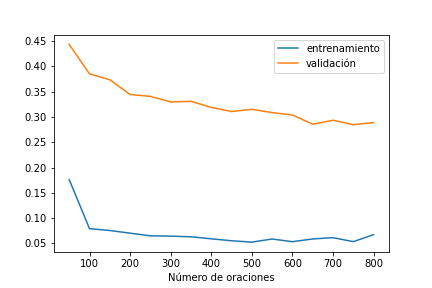
\includegraphics[width=\linewidth]{Graphics/learning_curves_relations.png}
		\caption{Modelo de Extracción de Entidades.}
	\end{subfigure}%
	\begin{subfigure}{.5\linewidth}
		\centering
		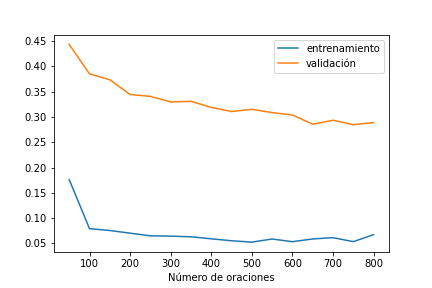
\includegraphics[width=\linewidth]{Graphics/learning_curves_relations.png}
		\caption{Modelo de Extracción de Relaciones.}
	\end{subfigure}
	\caption{Curvas de aprendizaje de los modelos, obtenidas a partir de la función de pérdida correspondiente. } \label{fig:learning_curves}
\end{figure}

Por su parte, la imagen \ref{fig:color_scaled_train_graphs} ilustra como el proceso de sobreajuste se reduce en ambos modelos a medida que crece el tamaño del conjunto de datos de entrenamiento.
Las curvas se corresponden con el comportamiento de la función de pérdida en los modelos a medida que avanza el proceso de entrenamiento.
Con respecto a la escala de colores, las tonalidades más oscuras indican mayor cantidad de ejemplos entrenantes.

\begin{figure}[h!]
	\centering
	\begin{subfigure}{.5\linewidth}
		\centering
		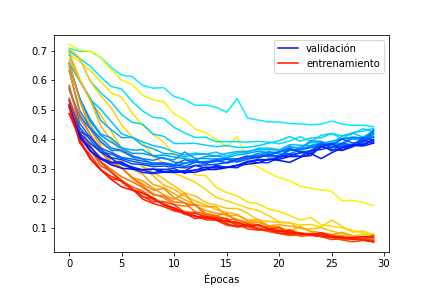
\includegraphics[width=\linewidth]{Graphics/color_scaled_train_graphs.png}
		\caption{Modelo de Extracción de Entidades.}
	\end{subfigure}%
	\begin{subfigure}{.5\linewidth}
		\centering
		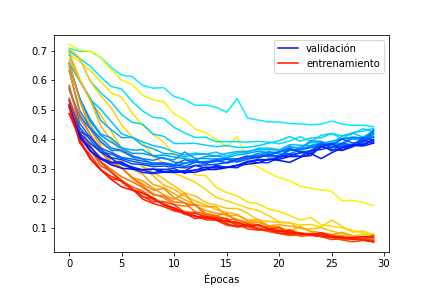
\includegraphics[width=\linewidth]{Graphics/color_scaled_train_graphs.png}
		\caption{Modelo de Extracción de Relaciones.}
	\end{subfigure}
	\caption{Sobreajuste de modelos entrenados con distinto núemero de casos entrenantes.. } \label{fig:color_scaled_train_graphs}
\end{figure}


Los experimentos se realizaron utilizando las colecciones de entrenamiento y desarrollo del evento correspondiente al año 2020.


\subsection{Análisis Ablasivo}

Con el objetivo de medir la influencia de las representaciones distribuidas empleadas, se realizó un análisis ablasivo sobre las distintas componentes de la entrada de los modelos.
Las tablas \ref{table:ablation_entities} y \ref{table:ablation_relations} resumen el desempeño de las distintas configuraciones consideradas.

\begin{table*}[tb!]\centering	
	\begin{tabular}{|c|c|c|c|}
		\hline
		\textbf{Configuraciones} &  \textbf{Medida F1} & \textbf{Precisión} & \textbf{Recobrado} \\
		\hline
		\textbf{BERT+CH+POS+DEP+ENT} & \textbf{0.5987} & \textbf{0.6250} & \textbf{0.8143} \\
		\hline
		\hline
		WE+Ch+POS+Dep+Ent& 0.5191  & 0.4105 & 0.7058 \\
		BERT+POS+Dep+Ent & 0.5283 & 0.4279 & 0.6904 \\
		BERT+Ch+Dep+Ent & 0.5515 & 0.4947 & 0.6231 \\
		BERT+Ch+POS+Ent &	0.5269 & 0.4345 & 0.6692 \\
		BERT+Ch+POS+Dep &	0.5331 & 0.4482 & 0.6577 \\
		BERT &	0.5204 & 0.5902 & 0.4654 \\
		\hline
	\end{tabular}
	\caption{Análisis ablasivo de sobre los componentes de la entrada. Modelo de extracción de entidades.\label{table:ablation_entities}}
\end{table*}

\begin{table*}[tb!]\centering
	\begin{tabular}{|c|c|c|c|}
		\hline
		\textbf{Configuraciones} &  \textbf{Medida F1} & \textbf{Precisión} & \textbf{Recobrado} \\
		\hline
		\textbf{BERT+CH+POS+DEP+ENT} & \textbf{0.5987} & \textbf{0.6250} & \textbf{0.8143} \\
		\hline
		\hline
		WE+Ch+POS+Dep+Ent& 0.5191  & 0.4105 & 0.7058 \\
		BERT+POS+Dep+Ent & 0.5283 & 0.4279 & 0.6904 \\
		BERT+Ch+Dep+Ent & 0.5515 & 0.4947 & 0.6231 \\
		BERT+Ch+POS+Ent &	0.5269 & 0.4345 & 0.6692 \\
		BERT+Ch+POS+Dep &	0.5331 & 0.4482 & 0.6577 \\
		BERT &	0.5204 & 0.5902 & 0.4654 \\
		\hline
	\end{tabular}
	\caption{Análisis ablasivo de sobre los componentes de la entrada. Modelo de extracción de relaciones.\label{table:ablation_relations}}
\end{table*}

Los experimentos fueron realizados utilizando los datos del evento correspondiente al año 2020.

\subsection{Hipótesis del Árbol de Dependencias}

En el caso del modelo para la extracción de relaciones, se evaluaron adicionalmente las hipótesis sobre el árbol de dependencias.
Para ello se entrenó un modelo con una complejidad semejante en términos de parámetros.
Se sustiuyó el camino en el árbol de dependencias por la secuencia de palabras de la oración completa, y se cambió el procesamiento mediante Tree-LSTM del subárbol relevante a las entidades, por una codificación basada en BiLSTM de las palabras que forman parte de las mismas.
Este modelo tiene un total de 709331 parámetros, cifra cercana a los 689713 parámetros del modelo basado en estructuras de dependencias.

La tabla \ref{table:dep_tree_hip} muestra una comparación del desempeño de las dos variantes, en el entorno del evento correspondiente al año 2020. Se incluyen los resultados obtenidos por otros participantes como referencia.

\begin{table*}[tb!]\centering
	\begin{tabular}{|c|c|c|c|}
		\hline
		&  \multicolumn{3}{c|}{\textbf{Escenario 3 (B)}} \\
		\hline
		\textbf{Equipo} & \textbf{F1} & \textbf{Precision} & \textbf{Recobrado} \\
		\hline
		IXA-NER-RE & 0.633235 & 0.647887 & 0.619231 \\
		\textbf{UH-MAJA-KD} & \textbf{0.59879} & \textbf{0.629237} & \textbf{0.571154} \\
		Vicomtech & 0.583243 & 0.671679 & 0.515385 \\
		Talp-UPC & 0.574786 & 0.646635 & 0.517308 \\
		UH-MatCom & 0.545035 & 0.682081 & 0.453846 \\
		SINAI & 0.461725 & 0.627063 & 0.365385 \\
		\textbf{BiLSTM} & \textbf{0.4382} & \textbf{0.4026} & \textbf{0.4808} \\
		HAPLAP & 0.316418 & 0.327835 & 0.305769 \\
		ExSim & 0.131313 & 0.527027 & 0.075 \\
		baseline & 0.131313 & 0.527027 & 0.07 \\	
		\hline
	\end{tabular}
	\caption{Comparación del modelo que prescinde de las estructuras de dependencias~(etiquetado como \textbf{BiLSTM}) y el resto de los participantes en el evento \textit{eHealth-KD} 2020. \label{table:dep_tree_hip}}
\end{table*}

Como se puede observar, los resultados del modelo que no utiliza información de las estructuras de dependencias son significativamente peores que la propuesta inicial, con una diferencia aproximada de 0.16 unidades en cuanto a los valores de la medida F1 en el escenario 3 de evaluación.


\section{Discusión}
%%================
%El modelo presentado obtuvo resultados relevantes en los contextos de ambos eventos del \emph{eHealth-KD Challenge} (2019 y 2020). Esto constituye un m\'erito de por si, pues muestra resultados cercanos al estado del arte en el evento (PONER NOMBRE DEL EVENTO). Este sistema supera por completo al presentado anteriormente en la competencia del 2019(PONER REF) e incluso obtiene mejores resultados que el mejor sistema en dicha comptencia, el cual resuelve las tareas A y B en un \'unico sistema \emph{end-to-end}. Es natural pensar que un sistema que resuelva ambas tareas a la vez obtendr\'a mejor rendimiento en general, pues existe una estrecha interrelaci\'on entre ambas tareas, sin embargo el modelo presentado las resuelve por separado y obtiene resultados muy similares, lo que sugiere que un modelo que resuelva ambas tareas haciendo uso de las caracteristicas esenciales de los modelos presentados para resolver las tareas A y B respectivamente pueda obtener un mejor desempe~no y avanzar el estado del arte.
%
%Particularmente en el escenario 2 se puede apreciar como el sistema posee muy buenos resultados, siendo el mejor en el contexto de la competencia del 2019 y teniendo resultados competitivos en el 2020. El modelo presentado para resolver la Tarea A sugiere varios aspectos interesantes. En primer lugar, como se pudo observar a trav\'es de la experimentaci\'on, los embeddings contextuales para cada palabra construidos a partir del modelo preentrenado de \textbf{BERT} son rasgos de gran impacto en la resoluci\'on de la Tarea A(PONER REF AL ANALISIS ABLASIVO). A partir del an\'alisis ablasivo se puede notar como cada una de los features que forman parte de la entrada tienen importancia para obtener el mejor desempe~no. A pesar de que el modelo de \textbf{BERT} fue entrenado de forma bidireccional en un gran corpus con m\'ultiples lenguajes, a\'un asi no ha sido entrenado necesariamente en las oraciones que conforman el corpus del evento, por lo que los embeddings contextuales obtenidos de \textbf{BERT} no obtienen los mejores resultados, a pesar de contener mucha informaci\'on como se pudo apreciar en el experimento haciendo uso solamente del modelo preentrenado de \textbf{BERT} y las capas de \textbf{CRF} a\'un as\'i el uso de rasgos como los embeddings de caracteres y los embeddings de PosTag, mejoran el desempe\~no del sistema. De la misma forma a partir de las \emph{Stacked BiLSTM} se construyen embeddings contextuales que contienen m\'as informacion, pues adem\'as de hacer uso de los embeddings contextuales preentrenados con \textbf{BERT}, hace uso de los character embeddings y PosTag embeddings analizando la oraci\'on bidireccionalmente obteniendo mayor informaci\'on para cada palabra dependiente del contexto y consiguiendo a\'un m\'as complejos rasgos dependientes del contexto con la segunda \emph{BiLSTM}. Otra observaci\'on interesante durante la experimentaci\'on es que como se ha visto en el estado del arte el uso de Embeddings de Palabras para la representaci\'on de las mismas y contruir embeddings contextuales a partir de estas ha obtenido muy buenos resultados en muchos trabajos(PONER REF), pero a\'un as\'i los experimentos utilizando los embeddings contextuales preentrenados a partir de \textbf{BERT} en lugar de los Embeddings de Palabras obtienen mejores resultados que los experimentos realizados con los Embeddings de Palabras y combinando los embeddings contextuales de \textbf{BERT} con los Embeddings de Palabra(PENSAR EN COMO EXPLICAR ESTO).








%===================================================================

\backmatter

%===================================================================================
% Chapter: Conclusiones
%===================================================================================
\chapter*{Conclusiones}\label{chapter:conclusions}
\addcontentsline{toc}{chapter}{Conclusiones}

Este trabajo propone un sistema basado en aprendizaje profundo haciendo uso de t\'ecnicas presentes en el estado del arte para resolver las Tareas A y B de los eventos (PONER EVENTOS), relacionados con los problemas de \textbf{NER} y \textbf{RE}. El sistema propuesto se entrena y eval\'ua dentro del dominio de la salud, pero es generalizable a otros dominios. Entre las contribuciones fundamentales del trabajo destacan: (1) la implementaci\'on de un sistema de extracci\'on autom\'atica de las anotaciones desde oraciones en lenguaje natural; (2) el dise\~no de modelos para resolver las Tareas A y B respectivamente con resultados competitivos y similares al estado del arte; (3) el an\'alisis del impacto de algunas representaciones de la entrada resultados finales. 

El modelo presentado para resolver la Tarea A es un modelo h\'ibrido de capas de \emph{BiLSTM} apiladas como codificadores contextuales y una capa \textbf{CRF} como decodificador de etiquetas. Se utilizaron como representaciones distribuidas de la entrada \emph{Embeddings de Caracteres y Pos-Tag} y \emph{Embeddings Contextuales} obtenidos a partir de un modelo preentrenado de \textbf{BERT}. Cada una de las representaciones de la entrada tiene un impacto positivo en el desempe\'no del modelo, siendo el de mayor impacto los \emph{Embeddings Contextuales} de \textbf{BERT}. Este modelo obtiene los mejores resultados en el segundo escenario de la competencia del evento (Nombre del evento) en su edici\'on 2019 y al mismo tiempo resultados competitivos en su edici\'on del a\~no 2020.(FALTA ANNADIR LO DE LAS LEARNING CURVES).

(CONCLUSIONES DE LAS RELACIONES)

(CONCLUSIONES CONJUNTAS)

  
%===================================================================================
\bibliographystyle{plain}
\bibliography{Bibliography}


\end{document}